% Standalone companion document to the survey (main.tex). Build from report/ with ./build.sh, which compiles main.tex first
% so that cross-references into the survey (\S, Fig., Table numbers) resolve through xr-hyper and link to main.pdf.
\def\loadxrhyper{}          % tells preamble.tex to load xr-hyper before hyperref
% ---------- compact preamble ----------
\documentclass[9pt,a4paper]{extarticle}
\usepackage[a4paper,margin=13mm,top=15mm,bottom=16mm,headsep=4mm,footskip=7mm]{geometry}
\usepackage[T1]{fontenc}\usepackage[utf8]{inputenc}
\usepackage{newtxtext}  % Times, as in the ICML template
\usepackage[scaled=0.82]{sourcecodepro}
\usepackage{microtype}
\setlength{\emergencystretch}{2em} % let narrow columns wrap long tokens instead of overflowing
\usepackage{amsmath,amssymb}
\usepackage{newtxmath}   % matching Times math
\usepackage[table,dvipsnames]{xcolor}
\usepackage{booktabs,multicol,tabularx,makecell,array,longtable}
\renewcommand*\setemergencystretch[2]{\emergencystretch 2em} % multicol otherwise resets it to 4pt per column
\usepackage{graphicx}
\usepackage{enumitem}
\usepackage{titlesec}
\usepackage{fancyhdr}
\usepackage{caption}
\usepackage{tcolorbox}\tcbuselibrary{skins,breakable}
\usepackage{tikz}\usetikzlibrary{positioning,arrows.meta,shapes,calc,fit,backgrounds}
\usepackage{pgfplots}\pgfplotsset{compat=1.18}
\usepackage{fontawesome5}
\usepackage{ragged2e}
\usepackage{CJKutf8}\newcommand{\cjk}[1]{\begin{CJK*}{UTF8}{gbsn}#1\end{CJK*}}
\usepackage[colorlinks,linkcolor=linkc,urlcolor=linkc,citecolor=linkc]{hyperref}

% ---------- palette (dataviz reference palette) ----------
\definecolor{s1}{HTML}{2a78d6}\definecolor{s2}{HTML}{eb6834}\definecolor{s3}{HTML}{1baf7a}
\definecolor{s4}{HTML}{eda100}\definecolor{s5}{HTML}{e87ba4}\definecolor{s6}{HTML}{008300}
\definecolor{s7}{HTML}{6250d6}\definecolor{s8}{HTML}{e34948}
\definecolor{critical}{HTML}{d03b3b}\definecolor{good}{HTML}{0ca30c}\definecolor{warning}{HTML}{fab219}
\definecolor{ink}{HTML}{0b0b0b}\definecolor{ink2}{HTML}{52514e}\definecolor{ink3}{HTML}{8a8984}
\definecolor{surface}{HTML}{f6f5f2}\definecolor{rule}{HTML}{d9d8d2}\definecolor{linkc}{HTML}{1c5cab}
\colorlet{agA}{s1}\colorlet{agB}{s2}\colorlet{agC}{s3}\colorlet{agD}{s7}
\colorlet{agE}{s5}\colorlet{agF}{s4}\colorlet{agG}{s6}\colorlet{agH}{ink3}

% ---------- typography ----------
\setlength{\parindent}{0pt}\setlength{\parskip}{2.5pt plus 1pt}
\setlength{\columnsep}{6mm}
\linespread{0.98}
\titleformat{\section}{\Large\bfseries\color{ink}}{\thesection}{0.6em}{}
\titlespacing*{\section}{0pt}{9pt plus 2pt}{4pt}
\titleformat{\subsection}{\large\bfseries\color{ink}}{\thesubsection}{0.6em}{}
\titlespacing*{\subsection}{0pt}{7pt plus 2pt}{3pt}
\titleformat{\subsubsection}{\normalsize\bfseries\color{ink2}}{\thesubsubsection}{0.5em}{}
\titlespacing*{\subsubsection}{0pt}{5pt plus 1pt}{2pt}
\titleformat{\paragraph}[runin]{\bfseries\color{ink2}}{}{0pt}{}[.\ ]
\titlespacing*{\paragraph}{0pt}{3pt}{0.5em}
\setlist{nosep,leftmargin=1.2em,itemsep=1pt}
\captionsetup{font={small,color=ink2},labelfont=bf,skip=3pt}
\renewcommand{\arraystretch}{1.08}
\makeatletter\setlength{\@fptop}{0pt}\makeatother
\pagestyle{fancy}\fancyhf{}
\fancyhead[L]{\footnotesize\color{ink2}Failure-attribution datasets for LLM agents}
\fancyhead[R]{\footnotesize\color{ink2}\nouppercase{\leftmark}}
\fancyfoot[C]{\footnotesize\color{ink2}\thepage}
\renewcommand{\headrulewidth}{0.3pt}\renewcommand{\headrule}{\color{rule}\hrule width\headwidth height 0.3pt}

% ---------- helper macros ----------
\newcommand{\code}[1]{\texttt{\small\def\_{\textunderscore\allowbreak}#1}}  % underscores are break points
\newcommand{\chip}[2]{\tikz[baseline=(t.base)]\node[fill=#1!18,text=#1!60!black,rounded corners=2pt,inner xsep=3pt,inner ysep=1.5pt,font=\scriptsize\bfseries](t){#2};}
\newcommand{\okbadge}{\chip{good}{available}}
\newcommand{\gatedbadge}{\chip{warning}{gated}}
\newcommand{\nobadge}{\chip{critical}{not released}}
\newcommand{\partialbadge}{\chip{s7}{partial}}
\newcommand{\naturalbadge}{\chip{s3}{natural}}
\newcommand{\injected}{\chip{s2}{injected}}
\newcommand{\lbl}[1]{\chip{ink3}{#1}}

% key-value identity block
\newenvironment{identity}{\begin{tcolorbox}[enhanced,colback=surface,colframe=rule,boxrule=0.3pt,arc=1.5pt,left=4pt,right=4pt,top=3pt,bottom=3pt,fontupper=\small]\begin{tabular}{@{}>{\bfseries\color{ink2}}l@{\hskip 5pt}>{\RaggedRight}p{\dimexpr\linewidth-2.1cm}@{}}}{\end{tabular}\end{tcolorbox}}

% stats table wrapper
\newenvironment{statsbox}{\begin{tcolorbox}[enhanced,colback=white,colframe=rule,boxrule=0.3pt,arc=1.5pt,left=3pt,right=3pt,top=2pt,bottom=2pt,fontupper=\small]}{\end{tcolorbox}}

% ---------- trajectory rendering ----------
\newcommand{\trajfont}{\ttfamily\footnotesize} % font for the trajectory step boxes
\newcommand{\trajtask}[2]{%
\begin{tcolorbox}[enhanced,colback=s1!6,colframe=s1!60!black,boxrule=0.4pt,arc=1.5pt,left=4pt,right=4pt,top=2pt,bottom=2pt,fontupper=\footnotesize,
  title={\footnotesize\bfseries\faTasks\ Task \ifx\\#1\\\else\textnormal{\scriptsize(\code{#1})}\fi},coltitle=white,colbacktitle=s1!60!black,toptitle=1pt,bottomtitle=1pt]
#2
\end{tcolorbox}}
% \begin{trajstep}{idx}{agent}{color} body \end{trajstep}
\newenvironment{trajstep}[3]{%
\begin{tcolorbox}[enhanced,breakable,colback=white,colframe=#3!55,boxrule=0pt,leftrule=2.2pt,arc=0pt,left=4pt,right=3pt,top=1.5pt,bottom=1.5pt,before skip=1.5pt,after skip=1.5pt,
  fontupper=\trajfont\color{ink},overlay unbroken and first={\node[anchor=north west,fill=#3!18,text=#3!50!black,font=\scriptsize\bfseries,inner xsep=3pt,inner ysep=1pt,rounded corners=1.5pt] at ([xshift=2pt,yshift=-1pt]frame.north west){#1 \textperiodcentered\ #2};}]
\vspace{8pt}\par}{\end{tcolorbox}}
\newenvironment{faultystep}[3]{%
\begin{tcolorbox}[enhanced,breakable,colback=critical!5,colframe=critical,boxrule=0.5pt,leftrule=2.2pt,arc=0pt,left=4pt,right=3pt,top=1.5pt,bottom=1.5pt,before skip=1.5pt,after skip=1.5pt,
  fontupper=\trajfont\color{ink},overlay unbroken and first={\node[anchor=north west,fill=critical,text=white,font=\scriptsize\bfseries,inner xsep=3pt,inner ysep=1pt,rounded corners=1.5pt] at ([xshift=2pt,yshift=-1pt]frame.north west){\faExclamationTriangle\ #1 \textperiodcentered\ #2 \textperiodcentered\ ANNOTATED ERROR STEP};}]
\vspace{8pt}\par}{\end{tcolorbox}}
% \trajannotation{agent}{step}{category}{reason}{ground truth}{final output}{extra}
\newcommand{\trajannotation}[7]{%
\begin{tcolorbox}[enhanced,breakable,colback=critical!4,colframe=critical!70!black,boxrule=0.4pt,arc=1.5pt,left=4pt,right=4pt,top=2pt,bottom=2pt,fontupper=\footnotesize,
  title={\footnotesize\bfseries\faTag\ Annotation},coltitle=white,colbacktitle=critical!70!black,toptitle=1pt,bottomtitle=1pt]
\begin{tabular}{@{}>{\bfseries\color{ink2}}l@{\hskip 5pt}>{\RaggedRight}p{\dimexpr\linewidth-2.0cm}@{}}
Faulty agent & #1\\
Faulty step & #2\\
Category & #3\\
Reason & #4\\
Ground truth & #5\\
System output & #6\\
\ifx\\#7\\\else Other labels & #7\\\fi
\end{tabular}
\end{tcolorbox}}
% shrink a table to the line width only when it is too wide (font-independent)
\newsavebox{\fitboxsb}
\newcommand{\fitbox}[1]{\sbox{\fitboxsb}{#1}\ifdim\wd\fitboxsb>\linewidth\resizebox{\linewidth}{!}{\usebox{\fitboxsb}}\else\usebox{\fitboxsb}\fi}
\newcommand{\badgerow}[1]{{\raggedright\noindent#1\par}} % badge rows wrap instead of overflowing

\usepackage[numbers,sort&compress]{natbib}
\externaldocument{build/main_labels}[main.pdf]   % survey labels (ds:*, sec:*, fig:*) from build/main.aux minus its \bibcite lines (written by build.sh); links open main.pdf
\fancyhead[L]{\footnotesize\color{ink2}Research proposals on failure attribution in LLM agent systems}
\title{\vspace{-9mm}\LARGE Failure Attribution in LLM Agent Systems\\[3pt]\large A working definition and five research proposals}
\author{\normalsize Companion to the dataset survey \emph{Datasets for Failure Attribution in LLM Agent Systems}, 30 October 2026}\date{}
\begin{document}
\maketitle\vspace{-7mm}
\begin{tcolorbox}[enhanced,colback=surface,colframe=rule,boxrule=0.3pt,arc=1.5pt,left=5pt,right=5pt,top=3pt,bottom=3pt,fontupper=\small]
\textbf{Scope.} This document fixes a working definition of failure attribution as an interventional quantity and develops five research proposals that follow from it. It is the companion of the survey \code{main.pdf}, which describes the 21 datasets the proposals draw their evidence from. References of the form \S3.2, Fig.~4, Section~7 or Table~1 that do not resolve inside this document point into the survey; in the PDF they link to \code{main.pdf}. All data, notes and scripts are in \code{/dataDisk/home/thanhdo/failure-attribution-datasets/}.
\end{tcolorbox}
\vspace{-2pt}\tableofcontents

\section{Overview}\label{sec:future}

\begin{multicols}{2}
\paragraph{What this document contains} The survey leaves one definitional gap and five research questions behind it. The gap is treated first; the five proposals follow and build on each other.
\begin{itemize}[leftmargin=1.1em]
\item \textbf{Preliminaries} (Section~\ref{sec:future:prelim}) fix a working definition of failure attribution as an \emph{interventional} quantity, together with the two assumptions it needs and the data engine that every proposal uses.
\item \textbf{Proposal 1} (Section~\ref{sec:future:perturb}) \emph{measures} that quantity with counterfactual rollouts and learns to predict it without executing.
\item \textbf{Proposal 2} (Section~\ref{sec:future:unsup}) \emph{estimates} it from logs and outcomes alone, with no step label, through a hazard model.
\item \textbf{Proposal 3} (Section~\ref{sec:future:train}) \emph{uses} it as a training signal for the agent that produced the failure and asks how much attribution accuracy is worth.
\item \textbf{Proposal 4} (Section~\ref{sec:future:lifecycle}) looks \emph{between} the error and the outcome: how an error propagates, is absorbed or locks in, which is the regime the first three treat as a point event.
\item \textbf{Proposal 5} (Section~\ref{sec:future:reroll}) turns attribution into a \emph{decision}: from which step a failed generation should be re-rolled when both the success it buys and the tokens it spends count, posed first for a single model and one generation, where it is cheapest to measure.
\end{itemize}

\paragraph{How the proposals are written} Every proposal has the same nine parts, in the same order, so that they can be read side by side:
\begin{itemize}[leftmargin=1.1em]
\item \emph{Motivation}: the evidence from the surveyed data that opens the question;
\item \emph{Closest prior work}: what already exists and what it lacks;
\item \emph{Setting}: the objects the proposal needs, introduced where they are first used as boxed \textcolor{s1!65!black}{\textbf{definitions}} and \textcolor{warning!60!black}{\textbf{assumptions}};
\item \emph{Research questions}: stated as full sentences in a \textcolor{s7!65!black}{\textbf{purple box}} and numbered \RQ{$p$.$i$} for proposal $p$;
\item \emph{Experiments}: numbered \EXP{$p$.$j$}, each naming the research questions it answers, fully or in part;
\item \emph{Evaluation}: one table per proposal giving, for each experiment, the data (collected or released), the metrics and the baselines or reference values;
\item \emph{Feasibility with the surveyed data}, \emph{Pitfalls to design for} and \emph{What would count as a result}.
\end{itemize}
Table~\ref{tab:roadmap} places the five proposals on one line each.
\end{multicols}

\medskip\noindent\begin{minipage}{\linewidth}\centering\small
\begin{tabularx}{\linewidth}{@{}l >{\RaggedRight\hsize=1.35\hsize}X >{\RaggedRight\hsize=0.75\hsize}X >{\RaggedRight\hsize=0.9\hsize}X@{}}\toprule
Proposal & Question in one sentence & Supervision it needs & What it produces \\\midrule
1 Perturbation screens & How much does the outcome change when one step is repaired or corrupted, and can that change be predicted without running the system? & replayable environment, no human label & effect profiles $e_\tau$, fragility curves, a surrogate $f$ \\
2 Label-free hazard model & Where in a failed run is the fatal step, when only outcomes---or nothing---are known? & outcome labels or none & a step-hazard model $h_\theta$, an online monitor \\
3 Attribution as training signal & Does a better attributor make a better agent, and at what accuracy does it start to help? & a trainable policy and a replayable environment & the accuracy-to-value curve, culprit-only updates \\
4 Error lifecycle & When an error enters a run, is it detected, corrected, tolerated or fatal, and how fast? & injections with absorbed branches kept & fate distributions, lifetime curves, per-agent profiles \\
5 Restart frontier & From which step should a failed generation be re-rolled when both the success it buys and the tokens it spends count? & one model, automatic verifier, no label & restart profiles and costs, the frontier, a position rule and its predictor \\\bottomrule
\end{tabularx}
\captionof{table}{The five proposals. All of them measure or estimate the same object---the success probability of a prefix and how an intervention moves it---and all run on the data engine of Table~\ref{tab:engine}.}
\label{tab:roadmap}
\end{minipage}\medskip

\section{Preliminaries: a working definition of failure attribution}\label{sec:future:prelim}

\begin{multicols}{2}
\paragraph{Why a definition is needed} The four proposals need a target that stays fixed from one dataset to the next. The survey shows that the current targets do not:
\begin{itemize}[leftmargin=1.1em]
\item Every dataset defines its labelled step \emph{counterfactually}---``the earliest step such that, had it been correct, the run would have succeeded''---but only TraceElephant ever tests the counterfactual by re-execution (\S\ref{ds:traceelephant}).
\item The summary that is labelled differs: the earliest decisive step (Who\&When, TrajErrBench, LongRCA), the first \emph{unrecovered} failure (AgentRx), a set of steps with per-annotator votes (MP-Bench), every error span (TRAIL), three timestamps $t_{\mathrm{err}}/t_{\mathrm{lock}}/t_{\mathrm{obs}}$ (Failure-as-a-Process), a step with a tolerance span (SearchAuditBench) or a set of (edge, fault side, mode) triples (MegaRCA-Mix).
\item Humans do not agree on the proxy: exact-step agreement is 40.3\% in LongRCA, 77.9\% in AgentHallu and 91.2\% / 66.7\% on the two TrajErrBench domains; TraceElephant's round-1 Krippendorff's $\alpha$ for the step is 0.64; the blamed agent agrees between Who\&When and TraceElephant on only 18 of 86 paired tasks.
\end{itemize}
We therefore take the counterfactual itself as the definition and treat every human label as a noisy estimate of it.

\paragraph{Setting and notation} Four objects are used throughout the document.
\begin{itemize}[leftmargin=1.1em]
\item An agent system $\pi$ (single- or multi-agent, stochastic) interacts with an environment $\mathcal{E}$ on a task $x$ with an automatic success predicate $S\in\{0,1\}$ (ground-truth answer, unit tests, verifier).
\item A trajectory is $\tau=(s_1,\dots,s_T)$; step $s_t=(a_t,u_t,o_t)$ records the acting agent $a_t\in\mathcal{A}$, its output $u_t$ (message, tool call or code) and the resulting observation $o_t$ (tool result, page, test log). $\tau_{<k}$ is the prefix $(s_1,\dots,s_{k-1})$.
\item \emph{One step is one policy decision}: an agent output together with the observation it produced. Orchestrator bookkeeping, user turns and bare tool returns are context, not candidates; this removes the indexing differences catalogued in Section~\ref{sec:reco}.
\item $\mathrm{Roll}(\tau_{<k}\oplus s_k')$ is the random continuation obtained by restoring the state reached after $\tau_{<k}$, executing the (possibly modified) step $s_k'$ and letting $\pi$ and $\mathcal{E}$ run to termination; randomness comes from sampling in $\pi$ and from $\mathcal{E}$.
\end{itemize}

\begin{assumption}{Replayability}{replay}
The environment state after $\tau_{<k}$ can be restored exactly (container snapshot, sandbox seed, simulated user), so that $\mathrm{Roll}(\cdot)$ is a well-defined distribution over continuations.
\begin{itemize}[leftmargin=1.1em]
\item Live-web environments violate this. SymTrace's selective replay \cite{luan2026symtrace} serves the prefix from recorded tool returns, which restores the prefix exactly but leaves the continuation unreproducible; the authors note that temperature-0 calls to a hosted model do not guarantee determinism either.
\item Live-web cases are therefore excluded from the measured part of every proposal and used for transfer tests only.
\end{itemize}
\end{assumption}

\begin{assumption}{Fixed intervention vocabulary}{vocab}
Interventions come from a finite, declared set $\Delta=\Delta_{\mathrm{fix}}\cup\Delta_{\mathrm{inj}}$; each $\delta\in\Delta$ is a deterministic map $s_k\mapsto\delta(s_k)$ that changes exactly one step. Table~\ref{tab:vocab} lists a starting vocabulary. ``A change to a step'' without such a vocabulary is not a learnable object.
\end{assumption}

\begin{definition}{Intervention effect}{effect}
For a trajectory $\tau$, a step index $k$ and an intervention $\delta\in\Delta$, the \emph{baseline} and \emph{intervened success rates} are
\begin{align*}
p_0(\tau,k)&=\Pr\big[S(\mathrm{Roll}(\tau_{<k}\oplus s_k))=1\big],\\
p_\delta(\tau,k)&=\Pr\big[S(\mathrm{Roll}(\tau_{<k}\oplus\delta(s_k)))=1\big],
\end{align*}
and the \emph{effect} is $\phi(\tau,k,\delta)=p_\delta(\tau,k)-p_0(\tau,k)\in[-1,1]$.
\begin{itemize}[leftmargin=1.1em]
\item Both rates are estimated by $N$ independent rollouts; $p_0$ is estimated with the original step \emph{re-executed}, not read from the observed outcome, which makes the effect robust to run-to-run stochasticity.
\item A step $k$ is \emph{$\alpha$-decisive} for a failed $\tau$ if $\max_{\delta\in\Delta_{\mathrm{fix}}}\phi(\tau,k,\delta)\ge\alpha$, and \emph{$\alpha$-fragile} for a successful $\tau$ if $\min_{\delta\in\Delta_{\mathrm{inj}}}\phi(\tau,k,\delta)\le-\alpha$.
\end{itemize}
\end{definition}

\begin{definition}{Failure attribution}{fa}
For a failed trajectory $\tau$ the \emph{repair-effect profile} is
\[e_\tau(k)=\max_{\delta\in\Delta_{\mathrm{fix}}}\phi(\tau,k,\delta),\qquad k=1,\dots,T,\]
and \emph{failure attribution} is the estimation of $e_\tau$. For a threshold $\alpha\in(0,1]$ stated with every result, the labels used in the literature are summary statistics of the profile:
\begin{itemize}[leftmargin=1.1em]
\item \textbf{error set} $E_\alpha(\tau)=\{k:\ e_\tau(k)\ge\alpha\}$ --- the steps whose repair would have rescued the run;
\item \textbf{decisive step} $k^\star=\min E_\alpha(\tau)$ --- the earliest of them;
\item \textbf{lock-in} $k_{\mathrm{lock}}=\max E_\alpha(\tau)+1$ --- the first step from which no single-step repair recovers the run;
\item \textbf{responsible agent} $a^\star=a_{k^\star}$ --- the agent that emitted the decisive step; no separate ``who'' label is defined;
\item \textbf{fault side} --- whether the maximising $\delta$ at $k^\star$ acts on the output $u_k$ (model-side) or on the observation $o_k$ (tool- or environment-side).
\end{itemize}
\end{definition}

\paragraph{Correspondence with the surveyed labels}
\begin{itemize}[leftmargin=1.1em]
\item $k^\star$ is the target of Who\&When, TraceElephant, TrajErrBench, LongRCA, CORRECT-Error and the injected datasets, and the $t_{\mathrm{err}}$ of Failure-as-a-Process.
\item $E_\alpha$ is what MP-Bench's vote counts, AgentRx's failure events and TRAIL's error spans approximate; MP-Bench's per-step consensus rate is a human estimate of $e_\tau(k)$ itself.
\item $k_{\mathrm{lock}}$ is AgentRx's ``first failure from which the run never recovers'' and Failure-as-a-Process's $t_{\mathrm{lock}}$; $k_{\mathrm{lock}}-k^\star$ is that paper's fix window (median 1 step).
\item $a^\star$: the sender of the labelled step equals the responsible role in 99.2\% of LongRCA and 100\% of TracerTraj records, so defining the agent through the step loses nothing and removes the naming problems of Section~\ref{sec:reco}.
\item Fault side recovers MegaRCA-Mix's model / harness / environment / grader sides and the environment-caused failures that SearchAuditBench excludes.
\end{itemize}

\paragraph{What the definition is robust to}
\begin{itemize}[leftmargin=1.1em]
\item \emph{Annotator variance.} The target is measured, not adjudicated; a dataset whose ground truth depends on who labelled it cannot be a stable target across datasets.
\item \emph{Run-to-run stochasticity.} $p_0$ is re-estimated by re-execution, so a run that failed by chance has a small effect everywhere instead of a forced label.
\item \emph{Several causes.} The error set is graded by effect size; MP-Bench's 16\% single-step agreement becomes a property of the profile (several steps of comparable effect) rather than label noise.
\item \emph{Recovery.} Decisive step and lock-in come from one profile, so the two conventions in the literature are reconciled instead of chosen between.
\item \emph{Observation level.} The definition lives on the system, not on the log: output-only logs, LLM-call traces and span trees are different estimators of the same quantity, not different tasks.
\end{itemize}

\paragraph{What must be fixed for it to be well posed}
\begin{itemize}[leftmargin=1.1em]
\item \emph{The vocabulary $\Delta$} (Assumption~\ref{as:vocab}, Table~\ref{tab:vocab}). ``Had it been correct'' is not learnable until ``correct'' is an operation; results are reported per intervention. Errors with no single-step intervention---a wrong team composition before the log begins, which is where 20 of 126 Who\&When Algorithm-Generated labels sit (step~0)---are declared out of scope, not scored as zero.
\item \emph{$N$ and $\alpha$.} Effects are reported with intervals; $N=5$--$10$ rollouts separate an effect of 0.5 from 0 but not 0.1 from 0, so $\alpha$ is not set below the resolution that $N$ affords.
\end{itemize}

\paragraph{Proxies when replay is impossible}
\begin{itemize}[leftmargin=1.1em]
\item Live-web GAIA and AssistantBench runs and output-only logs violate Assumption~\ref{as:replay}. There the human decisive step is used as a proxy for $k^\star$, scored with exact match \emph{and} a $\pm k$ window, and the agreement figures above are quoted as its ceiling.
\item No method is evaluated on proxies alone: the replayable environments of the survey (SWE-bench and SWE-Bench~Pro, ALFWorld, WebShop, $\tau^2$-Bench, TravelPlanner, VitaBench, Terminal-Bench) carry the measured version; the proxies test transfer.
\end{itemize}
In one sentence: failure attribution is the estimation of a step-level repair-effect profile under a declared intervention set, and the decisive step, the error set, the lock-in point and the responsible agent are summary statistics of that profile.

\paragraph{The shared data engine} Every human-labelled dataset of the survey is a test set, and only four of the 21 ship trajectories with both outcomes. The measured parts of the four proposals are therefore \emph{collected}, not downloaded, on the systems of Table~\ref{tab:engine}:
\begin{itemize}[leftmargin=1.1em]
\item rows 1--5 are systems whose agent code and environment are public and replayable (Assumption~\ref{as:replay}), with a verifier that supplies $S$ for free;
\item each row names the released human labels that can score a result \emph{on that system}, so that no new annotation is needed;
\item row 6 (live web) supports recorded-prefix replay only and is used for transfer tests;
\item the same infrastructure---state restore and an LLM-call cache---serves the rollouts of Proposal~1, the corpora of Proposal~2, the restarts of Proposal~3 and the injections of Proposal~4, which is what makes the four proposals one programme rather than four.
\end{itemize}
\end{multicols}

\medskip\noindent\begin{minipage}{\linewidth}\centering\small
\begin{tabularx}{\linewidth}{@{}l l >{\RaggedRight}X@{}}\toprule
Set & Intervention $\delta$ & Definition (changes step $k$ only) \\\midrule
$\Delta_{\mathrm{fix}}$ & \textsc{oracle-action} & replace $u_k$ by the action a human/LLM with access to the ground truth deems correct at $k$ \\
 & \textsc{hint} & prepend to $u_k$'s context a one-sentence statement of the fact the step got wrong (SymTrace's suspicious-node intervention \cite{luan2026symtrace}) \\
 & \textsc{fix-observation} & replace a corrupted/empty $o_k$ (404, OCR failure, swallowed output) by the correct observation \\
 & \textsc{reassign} & let a different agent $a'\neq a_k$ produce step $k$ \\\midrule
$\Delta_{\mathrm{inj}}$ & \textsc{corrupt-output} & rewrite $u_k$ with a context-aware error of mode $m$ (the Aegis/Who\&When~Pro injectors) \\
 & \textsc{corrupt-observation} & perturb $o_k$ (wrong number, truncated page, failing tool) \\
 & \textsc{delete} & drop step $k$ and continue \\
 & \textsc{swap-agent} & route step $k$ to an agent not designed for it \\\bottomrule
\end{tabularx}
\captionof{table}{A starting intervention vocabulary $\Delta$ (Assumption~\ref{as:vocab}). Each entry is a deterministic transformation; what varies across rollouts is only the continuation.}
\label{tab:vocab}
\end{minipage}\medskip

\medskip\noindent\begin{minipage}{\linewidth}\centering\scriptsize
\setlength{\tabcolsep}{3pt}
\begin{tabularx}{\linewidth}{@{}>{\RaggedRight\hsize=1.15\hsize}X >{\RaggedRight\hsize=0.8\hsize}X >{\RaggedRight\hsize=0.65\hsize}X >{\RaggedRight\hsize=1.2\hsize}X >{\RaggedRight\hsize=1.2\hsize}X@{}}\toprule
System family (public agent code) & State restore for $\mathrm{Roll}$ & Verifier $S$ & Released labels usable as test set & Remark \\\midrule
1\ \ $\tau^2$-Bench airline / retail: tool-calling agent + simulated user (TrajErrBench, AgentRx) & reset of domain DB and user simulator; seeded & DB-state constraints & TrajErrBench 400 ($\kappa$ 0.91), AgentRx 29 & cheapest: 29 messages, 20\,k characters per run \\
2\ \ ALFWorld, WebShop: AgentDebug's modular ReAct agent & deterministic text simulators & task reward & AgentErrorBench 100 + 50 & 30-step cap; observations repeat the page \\
3\ \ SWE-bench Verified / Pro, Terminal-Bench 2: SWE-Agent with TraceElephant's tracing middleware, OpenHands, mini-SWE-agent, Terminus~2 & container snapshot (Harbor) & hidden tests & TraceElephant 44, TrajErrBench 86, Failure-as-a-Process $t_{\mathrm{err}}/t_{\mathrm{lock}}$ for 1,184 runs once re-joined with the CodeTracer release & long: 120--300 steps, 200\,k characters; dominates the budget \\
4\ \ MASLab systems (LLM Debate, MacNet, AgentVerse, DyLAN, SmolAgents, Magentic-One) on GSM8K / MATH / HumanEval / MMLU-Pro: Aegis wrappers and injection factory; MetaGPT / AFlow runs of TracerTraj & no environment state; LLM-call cache, temperature 0 & answer match, unit tests & Aegis 600 (agent + mode, no step), TracerTraj test 790 (synthetic) & injector released; the natural setting for $\Delta_{\mathrm{inj}}$ with absorbed branches kept \\
5\ \ WebArena (Verified), AgentBench-OS, BIRD: HORIZON agents; LongRCA's planner--surfer--verifier controller & docker reset per task & environment verifier & HORIZON 294 judge step labels, LongRCA WebArena 177 & HORIZON agents public; LongRCA system code not released \\
6\ \ Live-web GAIA / AssistantBench / BrowseComp: Magentic-One, CaptainAgent, smolagents, deep-search scaffolds & none (recorded-prefix replay only) & answer match & Who\&When 184, TraceElephant 176, MP-Bench 289, SymFail 536, TRAIL 117, AgentHallu 36, SearchAuditBench 1,243 & Assumption~\ref{as:replay} fails: transfer tests only \\\bottomrule
\end{tabularx}
\captionof{table}{The data engine shared by the four proposals: systems of the survey on which unlabelled trajectories can be collected with replay, the verifier that gives the outcome for free, and the released labels that score the result on them. One thousand runs of one system cost about $1{,}000\times30$ steps $\times\,5$\,k tokens $\approx1.5\times10^{8}$ tokens with an open model.}
\label{tab:engine}
\end{minipage}\medskip

\section{Proposal 1: Counterfactual perturbation screens on agent trajectories}\label{sec:future:perturb}

\begin{multicols}{2}
\paragraph{Motivation} Every dataset in this survey defines the decisive step counterfactually, but only TraceElephant verifies the counterfactual by re-execution, and the injected datasets (Who\&When~Pro, Aegis, TracerTraj, CORRECT-Error) keep only the injections that produced a failure. Five observations from the raw data make the gap concrete:
\begin{itemize}[leftmargin=1.1em]
\item \emph{The root cause is run-specific.} Same task, same system family, re-run: the blamed agent agrees between Who\&When and TraceElephant in only 18 of 86 paired runs.
\item \emph{Labels are never tested.} In LongRCA, 364 of 1,140 reasons state no causal link to the outcome, and roughly one in five blames ``redundant/duplicate'' work in runs that still produced a final plan.
\item \emph{Absorption is the common case.} Aegis reports that injections flip a successful run into a failure between 34\% (DyLAN) and 77\% (LLM Debate) of the time; no dataset records the absorbed branch.
\item \emph{Re-runs drift.} SymTrace \cite{luan2026symtrace} re-ran 54 successful MAS executions three times each and saw 39 of them fail at least once, while unguided reruns of failed executions reproduced the failure in only 67.97\% of attempts.
\item \emph{Recovery is large.} In the faulty-agent injections of \citet{huang2024resilience} a reviewing Inspector agent recovered up to 96.4\% of the injected errors.
\end{itemize}
Absorption and run-to-run drift are large effects, not noise. The proposal turns attribution from a human-labelled classification target into the \emph{interventional quantity} of Definition~\ref{def:effect}, measured by rollouts and then predicted.

\paragraph{Closest prior work} Five strands contain parts of the programme; none contains the quantity.
\begin{itemize}[leftmargin=1.1em]
\item \emph{Replay-based repair.} SymTrace \cite{luan2026symtrace} (\S\ref{ds:symtrace}) records a MAS execution, picks an \emph{anchor} node, serves every LLM and tool call before the anchor from the log and lets everything after it run live---the operational form of $\mathrm{Roll}(\tau_{<k}\oplus s_k')$. Its intervention augments the anchor's request with a category-specific repair instruction (the \textsc{hint} of Table~\ref{tab:vocab}). On SymFail (536 evaluator-confirmed failures of AG2, CrewAI and Magentic-One) this repairs 20.15\% of failures in one attempt, against 6.90\% for three unguided reruns and 3.7--4.3\% for self-reflection and critic-agent baselines.
\item \emph{What replay-based repair lacks.} SymTrace runs one temperature-0 continuation per intervention, so it observes a single draw from $p_\delta$; it takes the anchor from a symptom detector rather than estimating which step is worth intervening on; and it has no injection side.
\item \emph{Counterfactual attribution.} Causal Agent Replay \cite{shah2026car} states the same do-intervention-then-re-execute estimator with confidence intervals and a Monte-Carlo Shapley extension for interacting steps, but validates it only on synthetic structural causal models. Minimal repair families \cite{li2026mrfr} replay \emph{sets} of events and show that single-event replay misses repairs that are only jointly sufficient. EMFA \cite{liao2026emfa} verifies the candidates of an error-propagation model with counterfactual checks and is the current best step-level attributor on Who\&When (+3.45 / +4.40 pp on the two subsets); TraceElephant's dynamic setting (\S\ref{ds:traceelephant}) is the same idea with a replayable environment.
\item \emph{Recovery as a measured property.} \citet{huang2024resilience} inject faulty agents into six MAS and find that a hierarchical topology loses 5.5\% of performance versus 10.5--23.7\% for flat ones; the hallucination-cascade study of \citet{jamshidi2026cascade} finds net attenuation along three-agent chains (0.422 $\to$ 0.272); ToolMaze \cite{zhu2026toolmaze} scores a perturbation-recovery rate separately from task success. None ties recovery to a labelled step of a natural failure.
\item \emph{Infrastructure and training.} AgentRewind \cite{zhuang2026agentrewind} checkpoints agent context and environment state jointly---an implementation of Assumption~\ref{as:replay}; Agent-R \cite{yuan2025agentr} trains agents on trajectories spliced at the first erroneous step with a correct branch, i.e.\ it consumes exactly the (prefix, repaired step) pairs that the surrogate of \EXP{1.2} would predict.
\item \emph{Perturbation biology.} Perturb-seq \cite{dixit2016perturbseq} applies a library of CRISPR perturbations to a population of cells and reads out the phenotype of each cell; GEARS \cite{roohani2024gears} and scGen \cite{lotfollahi2019scgen} then predict the phenotype of \emph{unseen} perturbations, so that most of the screen runs in silico. Table~\ref{tab:analogy} maps the objects; the correspondence supplies replicate-based effect estimation, graded essentiality and buffering, and interaction effects between two perturbations.
\end{itemize}
What is missing from all of them is an effect size per (trajectory, step, intervention), estimated from repeated rollouts, on failed \emph{and} successful natural runs.
\end{multicols}

\begin{table}[h]\centering\small
\begin{tabularx}{\linewidth}{@{}>{\RaggedRight}X >{\RaggedRight}X >{\RaggedRight}X@{}}\toprule
Perturbation biology & Agent trajectories & Remark \\\midrule
cell with a genetic background & trajectory prefix $\tau_{<k}$ with restored state & the ``background'' includes the task, the system and the prior errors \\
CRISPR knockout / activation & \textsc{delete}, \textsc{corrupt-}$\ast$ / \textsc{hint}, \textsc{oracle-action} & loss- and gain-of-function interventions on one step \\
phenotype readout (expression, viability) & success predicate $S$, optionally the failure mode of the continuation & binary readout today; a richer readout is the new trajectory itself \\
replicate cells & $N$ independent rollouts & estimates $p_\delta$; biology has thousands of replicates, we have $N\approx 5$--$10$ \\
essential gene & $\alpha$-decisive step & graded by effect size, not by a single annotator \\
genetic buffering / robustness & absorbed injection ($\phi\approx0$ on a successful run) & the data Aegis and Who\&When~Pro discard \\
epistasis (double perturbations) & two-step interventions $(k_1,\delta_1),(k_2,\delta_2)$ & tests MP-Bench's claim of several independent causes; cf.\ minimal repair families \cite{li2026mrfr} and \RQ{4.7} \\
in-silico perturbation predictor (GEARS, scGen) & surrogate $f$ (Definition~\ref{def:surrogate}, \EXP{1.2}) & replaces most rollouts once calibrated \\\bottomrule
\end{tabularx}
\caption{Correspondence between pooled perturbation screens and interventional failure attribution. Where it breaks: a gene library is finite and fixed, whereas edits to a step are open-ended (hence Assumption~\ref{as:vocab}); cells are independent replicates, whereas rollouts share a prefix and a policy, so $N$ is chosen per prefix; a rollout costs tokens rather than reagents.}
\label{tab:analogy}
\end{table}

\begin{multicols}{2}
\paragraph{Setting} The objects are those of Section~\ref{sec:future:prelim}: effect $\phi$, profile $e_\tau$, decisive step $k^\star$ and lock-in $k_{\mathrm{lock}}$ (Definitions~\ref{def:effect} and \ref{def:fa}) under Assumptions~\ref{as:replay} and \ref{as:vocab}. Fig.~\ref{fig:perturb} shows the measurement. Two further objects are needed: a model that replaces the rollouts, and a curve that summarises the injection side.

\begin{definition}{Effect surrogate}{surrogate}
An \emph{effect surrogate} is a model $f(\tau_{<k},s_k,\delta)\approx p_\delta(\tau,k)$ that predicts the intervened success rate from the prefix, the step and the intervention \emph{without executing} a rollout. It is trained on Monte-Carlo estimates $\hat p_\delta$ and scored as a probabilistic predictor (Brier score, calibration, AUROC of $\{\phi\ge\alpha\}$), separately for $\delta\in\Delta_{\mathrm{fix}}$ and $\delta\in\Delta_{\mathrm{inj}}$.
\end{definition}

\begin{definition}{Fragility curve and point of no return}{fragility}
For a successful trajectory $\tau$, the \emph{fragility curve}
\[r(k/T)=\mathbb{E}_{\delta\in\Delta_{\mathrm{inj}}}\,p_\delta(\tau,k)\]
is the probability that an error injected at relative position $k/T$ is absorbed. The \emph{point of no return} is the first $k$ at which $r$ drops below a stated threshold; it is the interventional counterpart of Failure-as-a-Process's $t_{\mathrm{lock}}$ (\S\ref{ds:failure_as_process}). Per-agent and per-mode versions of $r$ condition on $a_k$ and on the injected mode $m$.
\end{definition}

Neither object asks for a binary answer: a single re-run is one Bernoulli draw from $p_\delta$, and Section~\ref{ds:traceelephant} shows that draws from the same prefix land on different failures. The topology comparison of \citet{huang2024resilience} and SymTrace's rerun regressions \cite{luan2026symtrace} are single points on fragility curves.
\end{multicols}

\begin{figure}[h]\centering
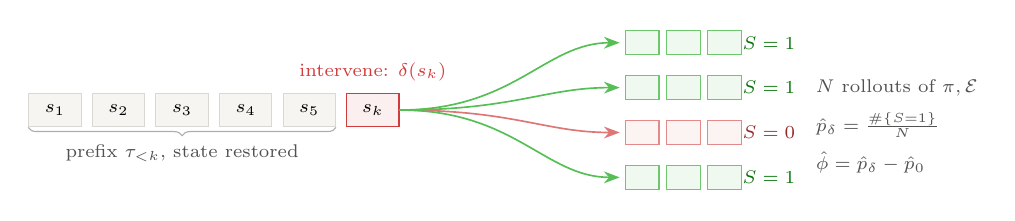
\begin{tikzpicture}[x=1cm,y=1cm,font=\scriptsize,>=Stealth,scale=0.95,every node/.style={transform shape}]
% prefix
\foreach \i in {1,...,5}{\node[draw=rule,fill=surface,minimum width=0.7cm,minimum height=0.45cm,inner sep=1pt] (s\i) at (\i*0.85,0) {$s_{\i}$};}
\node[draw=critical,fill=critical!8,minimum width=0.7cm,minimum height=0.45cm,inner sep=1pt] (sk) at (6*0.85,0) {$s_k$};
\node[above=1pt of sk,text=critical] {intervene: $\delta(s_k)$};
\draw[decorate,decoration={brace,amplitude=3pt,mirror},rule!80!black] (s1.south west) -- (s5.south east) node[midway,below=3pt,text=ink2]{prefix $\tau_{<k}$, state restored};
% rollouts
\foreach \j/\y/\c/\l in {1/0.9/good/$S=1$, 2/0.3/good/$S=1$, 3/-0.3/critical/$S=0$, 4/-0.9/good/$S=1$}{
  \draw[->,\c!70,line width=0.6pt] (sk.east) .. controls (7.0,0) and (7.4,\y) .. (8.4,\y);
  \foreach \i in {0,1,2}{\node[draw=\c!60,fill=\c!6,minimum width=0.45cm,minimum height=0.32cm,inner sep=0pt] at (8.7+\i*0.55,\y) {};}
  \node[right=2pt,text=\c!70!black] at (9.85,\y) {\l};}
\node[text=ink2,anchor=west] at (10.9,0.3) {$N$ rollouts of $\pi,\mathcal{E}$};
\node[text=ink2,anchor=west] at (10.9,-0.2) {$\hat p_\delta=\tfrac{\#\{S=1\}}{N}$};
\node[text=ink2,anchor=west] at (10.9,-0.7) {$\hat\phi=\hat p_\delta-\hat p_0$};
\end{tikzpicture}
\caption{The measured quantity (Definition~\ref{def:effect}). The state after the prefix is restored, step $k$ is replaced by $\delta(s_k)$, and $N$ independent continuations give a success rate; the same with the original $s_k$ gives the baseline. The effect is the difference.}
\label{fig:perturb}
\end{figure}

\begin{rqbox}{1}
\begin{description}[leftmargin=3.2em,style=sameline,font=\bfseries,itemsep=1.5pt]
\item[RQ\,1.1] Given a failed trajectory, which steps and which repair interventions raise the success probability of the continuation, and by how much? That is, what is the profile $e_\tau$, and which $(k,\delta)$ maximise $\phi$?
\item[RQ\,1.2] Given a successful trajectory, at which steps does an injected error cascade into failure rather than being absorbed, i.e.\ which steps are load-bearing?
\item[RQ\,1.3] Can the intervention effect be predicted from the prefix, the step and the intervention without executing a rollout, and is the prediction calibrated enough to replace most of the screen?
\item[RQ\,1.4] Do effect-based decisive steps agree with the human labels of the surveyed benchmarks, and where they disagree, which side do the rollouts support?
\item[RQ\,1.5] How far into a run can an agent system still recover from an injected error, how does that depend on the agent and the error mode, and do verifier agents change it?
\end{description}
\end{rqbox}

\begin{multicols}{2}
\paragraph{Experiments}
\begin{description}[leftmargin=1.4em,style=nextline,itemsep=1pt]
\item[\EXP{1.1} --- The screen (answers \RQ{1.1}, \RQ{1.2}).] Collect natural failed and successful trajectories on the replayable systems of Table~\ref{tab:engine}; for each, intervene at the human-labelled step (failures) or at stratified positions (successes) plus four control positions, with two interventions from each of $\Delta_{\mathrm{fix}}$ and $\Delta_{\mathrm{inj}}$ and $N=8$ rollouts per cell; estimate $\hat p_0$, $\hat p_\delta$ and $\hat\phi$ with intervals. Every continuation is stored with its outcome, which is the raw material of Proposals 2 and 4.
\item[\EXP{1.2} --- The surrogate (answers \RQ{1.3}).] Fit the effect surrogate $f$ of Definition~\ref{def:surrogate} on the output of \EXP{1.1} and test it on held-out prefixes, held-out tasks and held-out systems. Baselines: process-reward-model value estimates \cite{wang2024mathshepherd}, the system's own self-monitoring signals (orchestrator ledger flags precede the labelled step in 24 of 90 Magentic-One traces, \S\ref{ds:traceelephant}) and per-source position priors.
\item[\EXP{1.3} --- Attribution by effect (answers \RQ{1.4}).] Predict $k^\star=\arg\max_k e_\tau(k)$ from the screen and compare with the human labels of Who\&When, TraceElephant, MP-Bench and LongRCA and with the single-rollout counterfactual verifiers of EMFA and Causal Agent Replay \cite{liao2026emfa,shah2026car}. Disagreements between effect-based and human labels, adjudicated by further rollouts, are the interesting output; MP-Bench's three annotators make it possible to ask whether effect size tracks annotator consensus.
\item[\EXP{1.4} --- Fragility and lock-in (answers \RQ{1.5}).] From the injection half of \EXP{1.1}, estimate the fragility curve $r(k/T)$ of Definition~\ref{def:fragility} per system, per agent and per injected mode, and its point of no return; compare systems with and without a verifier agent and compare topologies as in \citet{huang2024resilience}. Proposal~4 refines this experiment by keeping the absorbed branches and labelling what happened to the error.
\end{description}
\end{multicols}

\medskip\noindent\begin{minipage}{\linewidth}\centering\scriptsize
\setlength{\tabcolsep}{3pt}
\begin{tabularx}{\linewidth}{@{}l >{\RaggedRight\hsize=1.25\hsize}X >{\RaggedRight\hsize=0.95\hsize}X >{\RaggedRight\hsize=0.8\hsize}X@{}}\toprule
Exp. & Data & Metrics & Baselines / reference values \\\midrule
\EXP{1.1} & \emph{Collected}: 200 failed + 200 successful runs on rows 1--5 of Table~\ref{tab:engine}, prefixes restored by snapshot; interventions from Table~\ref{tab:vocab}, $N=8$. Failed runs taken from the released labelled sets on the same systems (TraceElephant SWE-Agent 44, TrajErrBench 486, AgentErrorBench 200) so that a human label exists per run. & effect $\hat\phi$ with Wilson intervals; fraction of labelled steps that are $\alpha$-decisive at $\alpha\in\{0.25,0.5\}$; fraction of injections absorbed; share of labels outside the vocabulary (declared out of scope) & no baseline (measurement); SymTrace single-rerun repair 20.15\% and rerun reproduction 67.97\% \cite{luan2026symtrace}; Aegis absorption 23--66\% \\
\EXP{1.2} & \emph{Train}: $(\tau_{<k},s_k,\delta,\hat p_\delta)$ tuples of \EXP{1.1}; \emph{test}: held-out prefixes, tasks and systems; transfer to live-web runs (row 6) scored against human labels only & Brier score, expected calibration error, AUROC of $\{\phi\ge\alpha\}$; reported separately for $\Delta_{\mathrm{fix}}$ and $\Delta_{\mathrm{inj}}$; rollouts saved at fixed accuracy & PRM value estimates \cite{wang2024mathshepherd}; ledger flags; position priors (first step, last decision step, per-source histogram) \\
\EXP{1.3} & \emph{Test}: human labels of Who\&When, TraceElephant, MP-Bench, LongRCA on the replayable subset; MP-Bench per-step votes & exact and $\pm k$ agreement between $k^\star$ and the human step; nDCG@5 of $e_\tau$ against MP-Bench consensus; rank correlation of effect size with vote count; share of disagreements resolved by rollouts in favour of each side & EMFA and Causal Agent Replay single-rollout verifiers \cite{liao2026emfa,shah2026car}; human--human agreement (40.3\% LongRCA, $\alpha$ 0.64 TraceElephant) as the ceiling \\
\EXP{1.4} & \emph{Collected}: successful runs of \EXP{1.1} (TraceElephant withholds its 160 successes; Failure-as-a-Process PASS runs once re-joined) & $r(k/T)$ with intervals per system, agent and mode; point of no return at threshold 0.5; area under $r$ as a scalar robustness score & natural $t_{\mathrm{lock}}$ distribution of Failure-as-a-Process; hierarchical-vs-flat loss of \citet{huang2024resilience}; SymTrace rerun regressions \\\bottomrule
\end{tabularx}
\captionof{table}{Evaluation of Proposal 1: data, metrics and baselines per experiment.}
\label{tab:eval_p1}
\end{minipage}\medskip

\begin{multicols}{2}
\paragraph{Evaluation: data and metrics} Table~\ref{tab:eval_p1} lists them per experiment; three conventions apply throughout.
\begin{itemize}[leftmargin=1.1em]
\item \emph{Everything is probabilistic.} $p_0$ for a failed run is not zero (6.90\% of failed runs pass within three unguided reruns \cite{luan2026symtrace}), so effects carry intervals and the surrogate is scored as a probability, not a classification.
\item \emph{Human labels are references, not ground truth.} \EXP{1.3} reports agreement \emph{and} the adjudicated disagreements; the human--human agreement figures of Section~\ref{sec:future:prelim} are quoted as the ceiling.
\item \emph{Stratify by position and length.} Every curve is reported against $k/T$, and the rollout budget is stratified by trajectory length so that LongRCA-scale runs do not dominate.
\end{itemize}

\paragraph{Feasibility with the surveyed data}
\begin{itemize}[leftmargin=1.1em]
\item \emph{Environments.} Assumption~\ref{as:replay} holds for rows 1--5 of Table~\ref{tab:engine}: SWE-bench / SWE-Bench~Pro (TraceElephant's SWE-Agent runs, TrajErrBench), ALFWorld and WebShop (AgentErrorBench), the TravelPlanner and VitaBench sandboxes (LongRCA) and $\tau^2$-Bench with its simulated user (TrajErrBench, AgentRx). Live-web GAIA tests only the surrogate's transfer. SymTrace's recorded-prefix replay admits WebArena-Verified and AssistantBench runs at the price of an unreproducible continuation; AgentRewind's joint checkpoints \cite{zhuang2026agentrewind} restore the state after $\tau_{<k}$ cheaply.
\item \emph{Injectors.} Injectors for $\Delta_{\mathrm{inj}}$ exist (Aegis, Who\&When~Pro, TracerTraj) and only need to be run with the negatives retained.
\item \emph{Budget.} 400 trajectories, five positions, two interventions each and $N=8$ rollouts is $\approx$25\,k continuations; at the tail lengths observed here (medians of 10--145 steps, 30\,k--260\,k tokens per full trace) this is of the order of $10^9$ tokens, affordable with small open models and well below the cost of the human annotation it replaces.
\end{itemize}

\paragraph{Pitfalls to design for}
\begin{itemize}[leftmargin=1.1em]
\item \emph{Stochasticity.} A single temperature-0 replay, as in SymTrace, EMFA and the minimal-repair-family search, is one Bernoulli draw; 39 of 54 successful runs fail at least once in three reruns \cite{luan2026symtrace}.
\item \emph{Exposed downstream errors.} A repair at $k$ can succeed up to step $k+m$ and then fail for a new reason; each rollout is re-attributed (cheaply, by the surrogate) so that ``no flip'' separates into ``wrong step'' and ``several independent errors''.
\item \emph{Oracle fixes leak the answer.} \textsc{oracle-action} is constructed from the ground truth but must not inject it verbatim; \textsc{hint} is the weaker, safer variant and both are reported.
\item \emph{Vocabulary coverage.} Labelled errors with no single-step intervention (20 of 126 Who\&When Algorithm-Generated labels sit on step~0) are declared out of scope rather than scored as zero effect.
\item \emph{Cost concentration.} Long-horizon sources dominate the token budget; stratify the rollout budget by trajectory length rather than by trajectory.
\end{itemize}

\paragraph{What would count as a result}
\begin{itemize}[leftmargin=1.1em]
\item A calibrated surrogate (\EXP{1.2}) that predicts, from the prefix alone, which steps of a failed run are worth repairing and which steps of a successful run are load-bearing.
\item Effect-based labels (\EXP{1.3}) that agree with human consensus where humans agree and resolve the cases where they do not.
\item Fragility curves (\EXP{1.4}) that characterise, for the first time with an interventional definition, how far into a run a multi-agent system can still recover from an error.
\end{itemize}
The first two reuse the benchmarks surveyed here as test sets; the third is new measurement that none of them currently supports.
\end{multicols}

\section{Proposal 2: Label-free attribution from the flow of trajectories}\label{sec:future:unsup}

\begin{multicols}{2}
\paragraph{Motivation} Every human-labelled dataset in this survey is a \emph{test} set; the only training-scale resources are injected (Section~\ref{sec:g2}) and carry the positional skew of Fig.~\ref{fig:errpos}. \citet{yeh2026oat} show that step labels can be dispensed with altogether.
\begin{itemize}[leftmargin=1.1em]
\item \textsc{Oat} fits a one-class model of \emph{successful} trajectories---about 100 of them, embedded step by step with an LLM and modelled by a neural controlled differential equation \cite{kidger2020ncde}---and flags the steps of a failed run that deviate from the learned dynamics.
\item On the authors' own tool-use set it reaches F1 0.44 against 0.21 for GPT-4o prompting, on Who\&When 0.23 against 0.15 for GPT-5, and it runs 200--5\,000$\times$ faster.
\item The signal comes from \emph{selection}, not from the dynamics. The paper's own ablations put an RNN next-step predictor close behind the CDE, and the whole out-of-distribution gain (+0.172 AUROC, at $-$0.028 in-domain) comes from the gated control path that suppresses atypical inputs. The agent's mistakes are samples from its own policy, so a density model of \emph{all} its trajectories would rate them as typical actions; only the contrast with the success-conditioned flow makes them visible.
\item Selecting successes already requires an outcome label per trajectory, after which \textsc{Oat} discards the failed half of the data.
\item Successful runs are not clean either: Failure-as-a-Process PASS runs contain 2.3 error events per 22.8 steps, all recovered (Table~\ref{tab:contam}), so ``success'' is a property of the trajectory, not of its steps.
\end{itemize}
The proposal asks what the principled estimator is at each level of supervision, down to none, and which errors remain identifiable there.

\paragraph{Closest prior work}
\begin{itemize}[leftmargin=1.1em]
\item \emph{One-class trajectory models.} \textsc{Oat} \cite{yeh2026oat} as above; Isolation Forest and one-class SVM on step embeddings are the classical versions and serve as baselines.
\item \emph{Monte-Carlo value estimation.} Process-reward models estimate the value of a prefix from the outcomes of sampled continuations \cite{wang2024mathshepherd}; applied to agent runs, this is the rollout-supervised level below.
\item \emph{Weak supervision.} Multiple-instance learning \cite{dietterich1997mil} with a bag label per trajectory, and positive--unlabelled learning \cite{elkan2008pu,kiryo2017nnpu} with a known class prior, are the two statistical frames for ``some step of this failed run was wrong''.
\item \emph{Change-point detection.} Bayesian online change-point detection \cite{adams2007bocpd} infers a switch between regimes without labels; it is the fully unsupervised level below.
\item \emph{Discrete-time survival analysis} supplies the likelihood that ties the step-level hazard to the trajectory-level outcome.
\end{itemize}
None of these has been fitted to agent trajectories with the outcome as the only supervision, and none has been compared with \textsc{Oat} on the same encoder.

\paragraph{Setting} The notation is that of Section~\ref{sec:future:prelim}. Three objects are introduced: the levels of supervision a corpus can carry, two assumptions about where errors sit, and the hazard model that links steps to outcomes.

\begin{definition}{Levels of supervision}{levels}
A corpus of trajectories carries one of four levels:
\begin{itemize}[leftmargin=1.1em]
\item \textbf{L2}: the step label $t^\star$ (every dataset of Sections~\ref{sec:g1}--\ref{sec:g4});
\item \textbf{L1$^{+}$}: the outcomes of several \emph{continuations of the same prefix}---rollouts under Assumption~\ref{as:replay}, or the two branches of a fault injection---without any human label;
\item \textbf{L1}: the outcome $S$ only, from the benchmark verifier, unit tests or a judge---free wherever the task has a ground truth;
\item \textbf{L0}: raw logs, neither $S$ nor $t^\star$.
\end{itemize}
\textsc{Oat} sits between L1 and L0: it uses $S$ to select the training set and then ignores it. The proposal is built at L1 and L1$^{+}$.
\end{definition}

\begin{assumption}{Sparse errors}{sparse}
The fraction $\varepsilon$ of erroneous steps is small in every trajectory, failed or not; Table~\ref{tab:contam} puts it between 1\% and 20\% on the surveyed data.
\end{assumption}

\begin{assumption}{Absorption}{absorb}
A trajectory fails if and only if it contains an error from which the run never recovers; the first such step $t^\star$ determines the outcome, and later steps, right or wrong, are not causal.
\begin{itemize}[leftmargin=1.1em]
\item In the terms of Definition~\ref{def:fa}, $t^\star$ is the lock-in point $k_{\mathrm{lock}}$ (AgentRx's first unrecovered failure, Failure-as-a-Process's $t_{\mathrm{lock}}$), not the decisive step $k^\star$, which precedes it by the fix window---median 1 step, but more than 10 in 239 of 1,184 runs (\S\ref{ds:failure_as_process}).
\item A model built on this assumption is therefore expected to sit late relative to decisive-step labels and is scored against both.
\item Proposal~4 relaxes the assumption by adding a recovery transition.
\end{itemize}
\end{assumption}

\begin{definition}{Step hazard}{hazard}
Let $h_t=h_\theta(\tau_{<t},s_t)\in[0,1]$ be the probability that step $t$ is the first unrecovered error given its prefix. Under Assumption~\ref{as:absorb} the outcome likelihood is the discrete-time survival model
\begin{align*}
P(S{=}1\mid\tau)&=\textstyle\prod_{t=1}^{T}(1-h_t),\\
P(S{=}0,\,t^\star{=}t\mid\tau)&=h_t\textstyle\prod_{s<t}(1-h_s),
\end{align*}
and the attribution is the posterior
\[P(t^\star{=}t\mid S{=}0,\tau)=\frac{h_t\prod_{s<t}(1-h_s)}{1-\prod_{s}(1-h_s)}.\]
The survival function $\bar S_t(\tau)=\prod_{s\le t}(1-h_s)$ is the probability that a run which has reached $\tau_{\le t}$ still succeeds.
\end{definition}

\emph{Link to Proposal 1.} $\bar S_t$ is a learned surrogate of the baseline success rate $p_0(\tau,t{+}1)$ of Definition~\ref{def:effect}, and the online lock-in estimate of \EXP{2.3} is the point of no return of Definition~\ref{def:fragility}. The two proposals share one object: the rollouts of Proposal~1 measure it, the model here predicts it from the log.

\emph{How each level fits $h_\theta$} (Fig.~\ref{fig:hazard}):
\begin{itemize}[leftmargin=1.1em]
\item \textbf{L2.} The posterior is supervised directly.
\item \textbf{L1$^{+}$.} A rollout from $\tau_{<k}$ is an ordinary L1 trajectory that shares its first $k-1$ steps with $\tau$ and enters the same likelihood. What it adds is \emph{identification}: two continuations of one prefix with different outcomes place the hazard at or after the branch point, and $N$ continuations give a direct target $\hat p_0$ for $\bar S_{k-1}$---the Monte-Carlo value estimation of process-reward models \cite{wang2024mathshepherd}. It is the only step-level supervision that costs no label, and it is exactly the by-product of \EXP{1.1}.
\item \textbf{L1.} $t^\star$ is marginalised out and $\theta$ maximises $\sum_\tau\log P(S_\tau\mid\tau)$ over \emph{all} trajectories: a failed run contributes ``some step was fatal'', a successful run ``no step was''. This is multiple-instance learning \cite{dietterich1997mil} with the survival link in place of the usual noisy-OR, or positive--unlabelled learning at step level \cite{elkan2008pu,kiryo2017nnpu} with class prior $\varepsilon$.
\item \textbf{L0.} $S$ is latent as well. The likelihood then needs a model of the steps themselves and becomes a \emph{change-point mixture}: every trajectory follows a shared pre-change dynamics $q_0(s_t\mid\tau_{<t})$---the dominant mode---up to $t^\star\in\{1,\dots,T,\infty\}$, after which a second regime $q_1$ applies; $t^\star$ and $S=\mathbb{1}[t^\star{=}\infty]$ are inferred jointly by EM or by Bayesian change-point detection \cite{adams2007bocpd}.
\end{itemize}
\textsc{Oat} is the special case in which $q_0$ is fitted on known successes and the posterior is replaced by a threshold on reconstruction error.

\emph{What synthetic data adds.} The injectors of Table~\ref{tab:vocab} ($\Delta_{\mathrm{inj}}$, released with Aegis, Who\&When~Pro and TracerTraj) produce from one successful run
\begin{itemize}[leftmargin=1.1em]
\item a failed continuation with a known perturbed step, and, as often as not (absorption 23--66\% in Aegis), a successful continuation that contains a step known to be wrong;
\item both enter the L1 likelihood as ordinary trajectories, so the corpus grows without a label;
\item the pair is the sharpest test of the thesis: a hazard model must put high posterior on the injected step of the failed branch and low cumulative hazard on the identical step of the absorbed branch, whereas any detector of deviation from the success flow sees the same step twice and must flag both.
\end{itemize}
\end{multicols}

\begin{table}[h]\centering\small
\begin{tabular}{@{}llrrr@{}}\toprule
Dataset & Error unit & per trajectory & steps per trajectory & $\varepsilon$ \\\midrule
LongRCA & root step & 1 & 156 & 0.6\% \\
Failure as a Process (FAIL) & $t_{\mathrm{err}}$ / error events & 1 / 2.5 & 41.7 & 2.4\% / 6.0\% \\
Failure as a Process (PASS) & recovered error events & 2.3 & 22.8 & 10.1\% \\
TraceElephant & decisive LLM call & 1 & 27.1 & 3.7\% \\
Who\&When & decisive step & 1 & 22.2 & 4.5\% \\
AgentRx (public subset) & failure events & 4.6 & 44.7 & 10.3\% \\
TRAIL & spans carrying $\ge$1 error & 577 of 4\,626 spans & 31.3 & 12.5\% \\
AgentHallu & responsible step & 1 & 7.5 & 13.3\% \\
MP-Bench ($\ge$2 of 3 votes) & flagged steps & 4.2 & 23.3 & 18.0\% \\\bottomrule
\end{tabular}
\caption{Step-level error rate $\varepsilon$ on the surveyed data (means from the statistics tables of Sections~\ref{sec:g1}--\ref{sec:g4}), the basis of Assumption~\ref{as:sparse}. Even under the most generous labelling, more than 80\% of the steps of a failed trajectory are correct, and successful trajectories contain recovered errors at a comparable rate.}
\label{tab:contam}
\end{table}

\begin{figure}[h]\centering
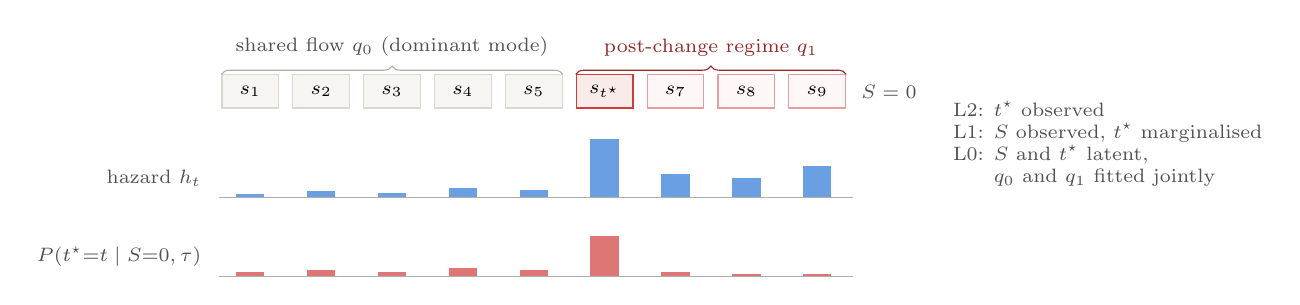
\begin{tikzpicture}[x=1cm,y=1cm,font=\scriptsize,>=Stealth]
\def\dx{0.9}
\foreach \i in {1,...,5}{\node[draw=rule,fill=surface,minimum width=0.72cm,minimum height=0.42cm,inner sep=1pt] (s\i) at (\i*\dx,0) {$s_{\i}$};}
\node[draw=critical,fill=critical!10,minimum width=0.72cm,minimum height=0.42cm,inner sep=1pt] (s6) at (6*\dx,0) {$s_{t^\star}$};
\foreach \i in {7,8,9}{\node[draw=critical!50,fill=critical!4,minimum width=0.72cm,minimum height=0.42cm,inner sep=1pt] (s\i) at (\i*\dx,0) {$s_{\i}$};}
\node[right=2pt of s9,text=ink2] {$S=0$};
\draw[decorate,decoration={brace,amplitude=3pt},rule!80!black] (s1.north west) -- (s5.north east) node[midway,above=3pt,text=ink2]{shared flow $q_0$ (dominant mode)};
\draw[decorate,decoration={brace,amplitude=3pt},critical!70!black] (s6.north west) -- (s9.north east) node[midway,above=3pt,text=critical!70!black]{post-change regime $q_1$};
\foreach \i/\h in {1/0.05,2/0.08,3/0.06,4/0.12,5/0.10,6/0.75,7/0.30,8/0.25,9/0.40}{
  \fill[s1!70] (\i*\dx-0.18,-1.35) rectangle (\i*\dx+0.18,-1.35+\h);}
\draw[rule!80!black] (0.5,-1.35) -- (9*\dx+0.45,-1.35);
\node[anchor=east,text=ink2] at (0.4,-1.1) {hazard $h_t$};
\foreach \i/\h in {1/0.053,2/0.080,3/0.055,4/0.104,5/0.076,6/0.520,7/0.052,8/0.030,9/0.036}{
  \fill[critical!70] (\i*\dx-0.18,-2.35) rectangle (\i*\dx+0.18,-2.35+\h);}
\draw[rule!80!black] (0.5,-2.35) -- (9*\dx+0.45,-2.35);
\node[anchor=east,text=ink2] at (0.4,-2.1) {$P(t^\star{=}t\mid S{=}0,\tau)$};
\node[anchor=north west,text=ink2,align=left] at (9*\dx+1.6,0.0) {L2: $t^\star$ observed\\L1: $S$ observed, $t^\star$ marginalised\\L0: $S$ and $t^\star$ latent,\\\phantom{L0: }$q_0$ and $q_1$ fitted jointly};
\end{tikzpicture}
\caption{The hazard model (Definition~\ref{def:hazard}). Each step receives a prefix-conditional hazard $h_t$; the survival product turns the hazards into an outcome probability (what L1 supervises) and, for a failed run, into a posterior over the first fatal step (the attribution). At L0 the same posterior is a change point between a shared dynamics $q_0$ and a post-error regime $q_1$.}
\label{fig:hazard}
\end{figure}

\begin{rqbox}{2}
\begin{description}[leftmargin=3.2em,style=sameline,font=\bfseries,itemsep=1.5pt]
\item[RQ\,2.1] Can a hazard model fitted on all trajectories of a corpus with outcome labels only, and no step label, match or exceed the one-class model \textsc{Oat} and prompted judges on the natural benchmarks when all use the same frozen step encoder?
\item[RQ\,2.2] How much does synthetic branching---several continuations of one prefix, or the two branches of an injection---add to step-level identification at zero label cost, and does the hazard model separate the injected step of a failed branch from the identical step of an absorbed branch?
\item[RQ\,2.3] Which error classes remain identifiable with no outcome label at all, from the dominant mode of the trajectory flow alone, and which do not?
\item[RQ\,2.4] Does the cumulative hazard of a prefix serve as an online monitor with positive lead time to the lock-in point, and how does it compare with the system's own self-monitoring signals?
\item[RQ\,2.5] How far does a model built on the absorption assumption sit from decisive-step labels as opposed to lock-in labels, and is the gap the fix window the natural data predict?
\end{description}
\end{rqbox}

\begin{multicols}{2}
\paragraph{Experiments}
\begin{description}[leftmargin=1.4em,style=nextline,itemsep=1pt]
\item[\EXP{2.1} --- Outcome-supervised hazard at L1 and L1$^{+}$ (answers \RQ{2.1}, \RQ{2.2}, \RQ{2.5}).] Fit $h_\theta$ by maximum likelihood on all trajectories of a corpus with outcomes, using the same frozen step embeddings as \textsc{Oat} so that the comparison isolates the estimator. The estimator is small: a causal GRU or two-layer transformer over the embeddings with a sigmoid hazard head, a sparsity prior on $\sum_t h_t$ (Assumption~\ref{as:sparse}) and the policy decision of Section~\ref{sec:future:prelim} as the step unit. Steps are discrete events, so no continuous-time machinery is needed; what matters is causality (prefix only) and sparsity. Fit once at L1 and once with the rollout prefixes of L1$^{+}$ added (the by-product of \EXP{1.1}), to measure what synthetic branching buys.
\item[\EXP{2.2} --- Injected-pair test (answers \RQ{2.2}).] Run the released injectors on successful runs with the absorbed branches kept, inject uniformly over positions (the released sets do not, Fig.~\ref{fig:errpos}) and hold out injected modes. Score the posterior on the injected step of the failed branch against the cumulative hazard on the same step of the absorbed branch; one-class detectors are expected to flag both alike.
\item[\EXP{2.3} --- Prefix monitor (answers \RQ{2.4}).] Because $h_t$ depends on the prefix only, the cumulative hazard $1-\prod_{s\le t}(1-h_s)$ is an online estimate of lock-in. Evaluate its lead time against $t_{\mathrm{lock}}$ and against the orchestrator's own ledger flags in Magentic-One traces (\S\ref{ds:traceelephant}). Proposal~4 (\EXP{4.7}) adds a delay guarantee to this monitor.
\item[\EXP{2.4} --- Fully unsupervised change-point model at L0 (answers \RQ{2.3}).] Same corpora, outcomes hidden. The question is not whether it beats \EXP{2.1}---it cannot---but which error classes are identifiable from the dominant mode alone. The generator-likelihood argument predicts that errors visible only in the action stream are not (a hallucinated summary is a typical summary), whereas errors that change the \emph{observation} stream are: tool exceptions, empty pages, repeated queries (MAST FM-1.3), stalled ledgers, premature termination. Fit $q_0$ on observations and on actions separately.
\end{description}
\end{multicols}

\medskip\noindent\begin{minipage}{\linewidth}\centering\scriptsize
\setlength{\tabcolsep}{3pt}
\begin{tabularx}{\linewidth}{@{}l >{\RaggedRight\hsize=1.25\hsize}X >{\RaggedRight\hsize=0.95\hsize}X >{\RaggedRight\hsize=0.8\hsize}X@{}}\toprule
Exp. & Data & Metrics & Baselines / reference values \\\midrule
\EXP{2.1} & \emph{Tier A, measured}: train and test in the same replayable system (rows 1--5 of Table~\ref{tab:engine}); $h_\theta$ fitted on self-collected runs, scored on TrajErrBench, AgentErrorBench and the SWE-Agent / SWE-Bench~Pro traces; on a subset the $\hat p_0$ curves of \EXP{1.1} are the reference for $\bar S_t$. \emph{Tier B, transfer}: frozen model on Who\&When (both subsets), MP-Bench, LongRCA, AgentRx and AgentHallu (whose 250 clean runs allow an L1 fit from its own logs). & exact and $\pm k$ step accuracy; distance to $t_{\mathrm{err}}$ and to $t_{\mathrm{lock}}$ reported separately (\RQ{2.5}); nDCG@5 against MP-Bench consensus; set-F1 over AgentRx events and TRAIL spans; $\pm5$ window on LongRCA; Brier score and calibration of $\bar S_t$ against $\hat p_0$ (Tier A only) and of $P(S{=}0\mid\tau)$ & position priors (first step, last decision step, per-source histogram); all-at-once prompting; \textsc{Oat} re-implemented on the same encoder; Isolation Forest and one-class SVM; value regression trained on rollouts only \cite{wang2024mathshepherd} (L1$^{+}$ without L1) \\
\EXP{2.2} & \emph{Tier C, exact labels}: Who\&When~Pro text split, CORRECT-Error, TracerTraj test as released; own injections on rows 1--5 with absorbed branches kept, uniform over position, modes held out & posterior mass on the injected step (failed branch) versus cumulative hazard at the same step (absorbed branch); AUROC of fatal-vs-absorbed; accuracy stratified by injected position and by held-out mode & one-class detectors (expected to flag both branches); injector position prior as a control \\
\EXP{2.3} & Failure-as-a-Process FAIL runs ($t_{\mathrm{lock}}$, 1,184) and PASS runs with recovered errors as hard negatives; Magentic-One traces with ledger flags & median lead time to $t_{\mathrm{lock}}$; precision and recall at fixed alarm thresholds; false-alarm rate on PASS runs & Failure-as-a-Process prompted monitor (82\% precision, 18\% recall, median lead time 0); ledger flags (precede the labelled step in 24 of 90 traces) \\
\EXP{2.4} & same corpora as \EXP{2.1} with outcomes hidden; taxonomy labels of TrajErrBench modules, Who\&When~Pro families, TRAIL and AgentRx categories & recall of the labelled step per error category, fitted on observations and on actions separately; the identifiability map is the result & \EXP{2.1} at L1 as the upper reference; \textsc{Oat} \\\bottomrule
\end{tabularx}
\captionof{table}{Evaluation of Proposal 2: data, metrics and baselines per experiment. Tiers A--C score the method where its target is measurable, where it must transfer and where labels are exact.}
\label{tab:eval_p2}
\end{minipage}\medskip

\begin{multicols}{2}
\paragraph{Evaluation: data and metrics} Table~\ref{tab:eval_p2} lists them per experiment; four conventions apply.
\begin{itemize}[leftmargin=1.1em]
\item \emph{Same encoder for every method.} Baselines, \textsc{Oat} and the hazard head share the frozen step embeddings, so differences are differences between estimators.
\item \emph{Two references per failed run.} Distance to $t_{\mathrm{err}}$ and to $t_{\mathrm{lock}}$ are reported separately, because Assumption~\ref{as:absorb} predicts a late bias against the former.
\item \emph{Robustness to outcome noise.} Outcome labels are flipped at rates up to the 12.9\% verifier--judge disagreement observed in HORIZON, and judge-only against verifier-only outcomes are compared on the same runs.
\item \emph{The injected sets are test sets.} Who\&When~Pro, CORRECT-Error and TracerTraj are used in Tier~C only, never for training, so that the injector's position prior is not learned.
\end{itemize}

\paragraph{Feasibility with the surveyed data}
\begin{itemize}[leftmargin=1.1em]
\item \emph{Released corpora with both outcomes.} AgentHallu (443 hallucinated / 250 clean), HORIZON (2\,498 / 1\,284 by judge), TRAIL (148 runs not selected by outcome) and Failure-as-a-Process (1\,184 / 610, annotations only---the CodeTracer trajectories must be re-joined). The core MAS benchmarks release failures only (TraceElephant withholds its 160 successful runs; Who\&When~Pro and Aegis do not ship their successful seeds).
\item \emph{Collection engine.} Everything else is collected on the systems of Table~\ref{tab:engine}, where the outcome is free; the same state restore and LLM-call cache serve the rollouts of Proposal~1.
\item \emph{Evaluation.} The set-labelled datasets for \EXP{2.1} and \EXP{2.4} and the three timestamps of Failure-as-a-Process for \EXP{2.3} exist already; no new annotation is needed.
\item \emph{Budget.} One forward pass per step for the embeddings: $\approx$2\,k trajectories $\times$ 30\,k tokens $\approx6\times10^{7}$ tokens, three to four orders of magnitude below the perturbation screen of Proposal~1; the hazard head trains in minutes.
\end{itemize}

\paragraph{Pitfalls to design for}
\begin{itemize}[leftmargin=1.1em]
\item \emph{The last-step shortcut.} The final answer reveals the outcome, so an L1 model will put hazard on it; the injected datasets show how strong that prior is (median relative position 0.83 in Who\&When~Pro, 0.95 in CORRECT-Error). Mask the last $k$ steps from the hazard input and report accuracy with the final step excluded.
\item \emph{Task difficulty as a confound.} Hard tasks produce both failures and unusual steps, so an outcome model can learn ``this task is hard'' instead of ``this step is wrong''. A matched design---the same task run to both outcomes---removes it; the 89 tasks $\times$ 21 systems of Section~\ref{ds:failure_as_process} are the template.
\item \emph{Recovered errors.} The survival likelihood tolerates them (a success only requires that no error was fatal); the plain multiple-instance assumption ``success bags are clean'' does not. Use the positive--unlabelled formulation with the prior from Table~\ref{tab:contam} when the any-error target is wanted; Proposal~4 makes recovered errors a target in their own right.
\item \emph{Identifiability and model selection at L0.} A change-point mixture can converge to a split that is not error-related (planning phase versus execution phase, say). Use a small L2 set for model selection and calibration only, never for training, and say so.
\item \emph{Anomaly is not causality.} Both \textsc{Oat} and \EXP{2.4} flag deviation; only the counterfactual rollouts of Proposal~1 can confirm that a flagged step is decisive. The two proposals close a loop: the hazard posterior is a cheap proposal distribution for where to intervene, and the rollouts return labels that re-fit $h_\theta$ at L2.
\end{itemize}

\paragraph{What would count as a result}
\begin{itemize}[leftmargin=1.1em]
\item An L1 estimator that matches or exceeds \textsc{Oat} and prompting on the natural benchmarks with the same encoder and no step labels, with a calibrated outcome probability as a by-product.
\item A measured gain from synthetic branching: the L1$^{+}$ fit beats the L1 fit on Tier~A at equal label cost (zero), and the hazard model separates injected from absorbed branches where one-class detectors cannot.
\item An identifiability map for L0: the error categories that can and cannot be recovered from the dominant mode, which tells practitioners what a label-free monitor will and will not catch.
\item A prefix monitor with positive median lead time to $t_{\mathrm{lock}}$.
\end{itemize}
\end{multicols}

\section{Proposal 3: Attribution-guided policy improvement}\label{sec:future:train}

\begin{multicols}{2}
\paragraph{Motivation} The datasets of this survey are built to score \emph{attributors}. The obvious consumer of a good attributor is the agent that produced the failure: a label $(a^\star,k^\star)$ says which parameters to move and from which state to try again. A literature search on this direction (notes in \code{notes/attribution\_as\_training\_signal.md}) gives three findings.
\begin{itemize}[leftmargin=1.1em]
\item \emph{The mechanism exists, under other names.} The strongest 2026 agent-RL methods locate a ``pivotal'', ``critical'' or ``irrecoverable'' step of a failed rollout and use it to restart rollouts there \cite{tian2026mirl,guo2026pivoarl,shi2026r3l,liu2026sprout,liang2026elpo}, to reweight the advantage at that step \cite{zhu2026fault,huang2026etro,jung2026prover,agentevolver2025,zhu2026lvrl} or to build preference pairs there \cite{li2026cso,yuan2025agentr,steca2025,cuarecovery2026}. None cites a failure-attribution benchmark as a source of signal, and none uses an attributor trained on one.
\item \emph{The benchmarks never close the loop.} Every downstream experiment inside an attribution paper is inference-time: AgenTracer feeds its tracer's reasoning back as a prompt for three rounds (gains of 4.8--14.2\%) \cite{agentracer2026}, AgentDebug re-rolls from the critical step with guidance \cite{agentdebug2026}, SearchAuditor resumes at the critical step with a repair directive \cite{searchauditor2026}, SymTrace replays one node \cite{luan2026symtrace}. No weights change. The only multi-agent blueprint---first-error localisation followed by preference pairs on the blamed agent---is a position paper without experiments \cite{yang2025blame}.
\item \emph{Attribution accuracy is never related to training value.} Nobody has asked whether a step metric from Sections~\ref{sec:g1}--\ref{sec:g4} predicts how much the agent improves when the label is used. The one direct measurement is negative: on 150 SWE-bench Verified runs, LLM-judge ``first mistake'' labels fall where the success probability does \emph{not} drop in 66\% of cases, only 7 of 188 judge answers name the decisive step, and restarting from the judge's step changes expected success by $-0.03$ to $-0.08$, whereas restarting from the certified point of no return raises it from 0.44 to 0.53 \cite{shen2026epv}. SearchAuditor's ablation adds that a generic hint at the predicted step repairs fewer failures (5.6\%) than an unguided retry (9.4\%), against 17.4\% with the auditor's directive \cite{searchauditor2026}: the location is necessary, not sufficient.
\end{itemize}
The pattern shared by the methods that work is \emph{propose, verify, then credit}: a judge or the policy proposes a step, a few current-policy continuations confirm that the outcome actually turns there, and only then does the step shape credit or data \cite{liang2026elpo,jung2026prover,li2026cso,chu2026agentgrad}. That verification step is the screen of Proposal~1 with $N$ between 1 and 8.

\paragraph{Closest prior work} Table~\ref{tab:entry} places the existing methods on the entry points defined below. Four groups:
\begin{itemize}[leftmargin=1.1em]
\item \emph{Restart methods} (MiRL, PivoARL, R$^3$L, SPROUT, ELPO) start the next rollouts from a chosen prefix; only ELPO verifies the prefix with rollouts, by binary search for the first irrecoverable step \cite{liang2026elpo}.
\item \emph{Credit methods} (FAULT, ETRO, ProVer, AgentEvolver, LVRL) reweight or truncate the advantage; ProVer verifies with $N=8$ continuations but uses positive segments only \cite{jung2026prover}.
\item \emph{Data methods} (CSO, Agent-R, CUA-Recovery) build a preference pair or a spliced correction at the step; CSO checks the alternative by policy continuation \cite{li2026cso}.
\item \emph{Multi-agent credit} (MAPPA, C3, AgentGrad) assigns per-agent credit from a coach, from counterfactual continuation of every message, or from sequential intervention, on two- to three-agent mathematics or on prompts only \cite{li2026mappa,chen2026c3,chu2026agentgrad}; nothing uses (agent, step) blame on a GAIA-style system.
\end{itemize}

\paragraph{Setting} The agent is a trainable policy $\pi_\theta$ (single- or multi-agent, each agent $a\in\mathcal{A}$ owning a parameter subset $\theta_a$) run on tasks with a success predicate $S$; the notation is that of Section~\ref{sec:future:prelim}.
\begin{itemize}[leftmargin=1.1em]
\item A group-relative outcome-only update (GRPO and its agentic variants \cite{feng2025gigpo}) applies to every step of a failed trajectory the same negative advantage $A_\tau<0$:
\[g^{\mathrm{unif}}_\tau=A_\tau\sum_{t=1}^{T}\nabla_\theta\log\pi_\theta(u_t\mid\tau_{<t}).\]
\item Under Assumption~\ref{as:absorb} only the steps in the error set are causal, so this estimator pushes down $T-|E_\alpha(\tau)|$ correct decisions per failed run; with the error rates of Table~\ref{tab:contam} that is 80--99\% of its negative gradient mass.
\item An \emph{attributor} $\mathcal{A}$ maps a trajectory to a non-negative weight vector $\hat w_\tau\in\mathbb{R}^T$, an estimate of where the causal mass lies: a point estimate $\hat w_\tau=\mathbb{1}[t=\hat k]$, a posterior $\hat w_\tau(t)=P(t^\star{=}t\mid S{=}0,\tau)$ from the hazard model of Definition~\ref{def:hazard}, or a graded profile $\hat w_\tau\propto\hat e_\tau$ from the screen of Definition~\ref{def:fa}.
\end{itemize}

\begin{definition}{Attribution-weighted update}{attrgrad}
Given $\hat w_\tau$ and a mixing weight $\lambda\in[0,1]$, the attribution-weighted policy gradient of a failed trajectory is
\[g^{\hat w}_\tau=A_\tau\sum_{t=1}^{T}\big[(1-\lambda)+\lambda\,T\hat w_\tau(t)/\|\hat w_\tau\|_1\big]\nabla_\theta\log\pi_\theta(u_t\mid\tau_{<t}),\]
so that $\lambda=0$ recovers $g^{\mathrm{unif}}_\tau$ and $\lambda=1$ with the true $w_\tau=\mathbb{1}[t=k^\star]$ concentrates the whole penalty on the decisive step. Successful trajectories are unchanged. The bias of $g^{\hat w}$ relative to the ideal $g^{w}$ is governed by the attributor's precision at the chosen tolerance---what the step metrics of this survey measure---and its variance reduction relative to $g^{\mathrm{unif}}$ by $1-\varepsilon$.
\end{definition}

\begin{definition}{Entry points}{entry}
The weight vector can enter training in four places (Fig.~\ref{fig:entry}):
\begin{itemize}[leftmargin=1.1em]
\item \textbf{R --- restart.} Rollouts for the next update start from $\tau_{<k}$ with $k\sim\rho_\tau\propto\hat w_\tau$ instead of from the task prompt. This reshapes the state distribution toward decisions that matter and lets a group of continuations share a prefix, so GRPO's within-group comparison becomes a step-level comparison at $k$. Needs Assumption~\ref{as:replay}.
\item \textbf{C --- credit.} The update of Definition~\ref{def:attrgrad}, optionally with \emph{truncation}: no dense supervision after $\hat k$, because later steps are conditioned on a state the current policy would not reach \cite{huang2026etro,guo2026pivoarl}. Needs only the log and an attributor.
\item \textbf{D --- data.} A preference pair or a spliced correction at $\hat k$: the policy's action against an alternative from which a continuation succeeds \cite{li2026cso}, or the failed prefix followed by a successful sibling branch \cite{yuan2025agentr}. Needs one rollout from $\tau_{<\hat k}\oplus\delta(s_{\hat k})$ with $\delta\in\Delta_{\mathrm{fix}}$.
\item \textbf{M --- culprit-only update} (multi-agent). $\hat w$ is indexed by (agent, step); the gradient is applied to $\theta_{a^\star}$ and the advantages of the other agents are masked, the weight-space analogue of intervention-guided prompt optimisation \cite{chu2026agentgrad}.
\end{itemize}
\end{definition}

\begin{definition}{Training value of an attributor}{trainval}
For a fixed recipe, budget $B$ of environment steps and seeds, let $\pi^{\mathcal{A}}_B$ be the policy after training with weights from $\mathcal{A}$ and $\pi^{\mathrm{unif}}_B$ the outcome-only policy at the same budget. The \emph{training value} is $V_B(\mathcal{A})=J(\pi^{\mathcal{A}}_B)-J(\pi^{\mathrm{unif}}_B)$, with $J$ the held-out success rate; the \emph{accuracy-to-value curve} is $V_B$ plotted against the attributor's step accuracy at the tolerance used by the recipe.
\end{definition}

\emph{The attributor ladder.} The experiments hold the training recipe fixed and vary only $\mathcal{A}$, ordered by cost and by how much of the outcome it has seen:
\begin{enumerate}[leftmargin=1.4em,itemsep=1pt]
\item \emph{position priors}: last decision step, per-source histogram (Proposal~2);
\item \emph{outcome variance, no attribution}: start states where the reference policy sometimes fails \cite{pivotrl2026};
\item \emph{the policy's own reflection} \cite{guo2026pivoarl};
\item \emph{prompted judge}: the all-at-once protocol of Who\&When with a frontier model;
\item \emph{trained attributors}: an 8B model trained on TracerTraj, Aegis or Who\&When~Pro with the AgenTracer recipe \cite{agentracer2026}, and the hazard model of Proposal~2 fitted at L1 on the same system's runs;
\item \emph{rollout-verified}: any of 3--5 followed by the screen of Proposal~1 with $N\le8$ at the proposed step and its neighbours \cite{liang2026elpo,jung2026prover};
\item \emph{oracle}: the rollout-measured $k^\star$ with large $N$, affordable only on a test subset.
\end{enumerate}
Each rung is scored twice: by the attribution metrics of this survey on held-out labels of the same system, and by its training value.
\end{multicols}

\begin{figure}[h]\centering
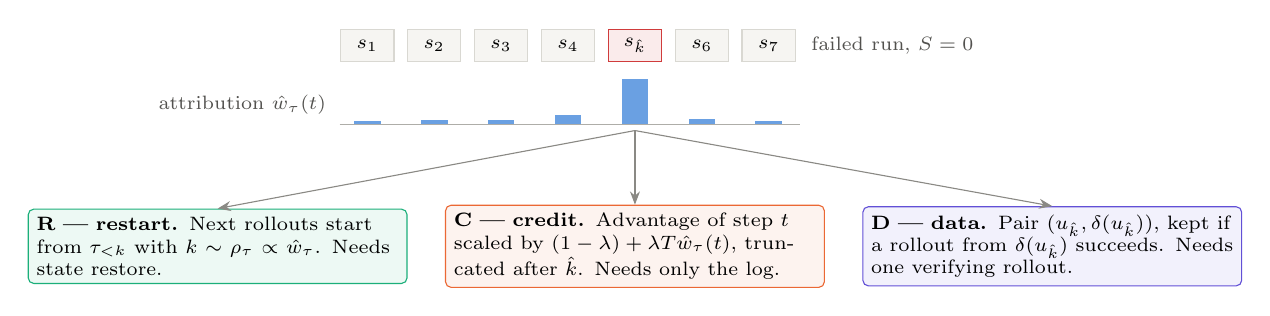
\begin{tikzpicture}[x=1cm,y=1cm,font=\scriptsize,>=Stealth]
\def\dx{0.85}
\foreach \i in {1,...,4}{\node[draw=rule,fill=surface,minimum width=0.68cm,minimum height=0.4cm,inner sep=1pt] (s\i) at (\i*\dx,0) {$s_{\i}$};}
\node[draw=critical,fill=critical!10,minimum width=0.68cm,minimum height=0.4cm,inner sep=1pt] (s5) at (5*\dx,0) {$s_{\hat k}$};
\foreach \i in {6,7}{\node[draw=rule,fill=surface,minimum width=0.68cm,minimum height=0.4cm,inner sep=1pt] (s\i) at (\i*\dx,0) {$s_{\i}$};}
\node[right=2pt of s7,text=ink2] {failed run, $S=0$};
\foreach \i/\h in {1/0.04,2/0.06,3/0.05,4/0.12,5/0.58,6/0.07,7/0.04}{\fill[s1!70] (\i*\dx-0.17,-1.0) rectangle (\i*\dx+0.17,-1.0+\h);}
\draw[rule!80!black] (0.5,-1.0) -- (7*\dx+0.4,-1.0);
\node[anchor=east,text=ink2] at (0.45,-0.75) {attribution $\hat w_\tau(t)$};
\coordinate (p) at (5*\dx,-1.08);
\node[draw=s3,fill=s3!8,rounded corners=2pt,inner sep=3pt,text width=4.6cm,align=left] (R) at (5*\dx-5.3,-2.55) {\textbf{R --- restart.} Next rollouts start from $\tau_{<k}$ with $k\sim\rho_\tau\propto\hat w_\tau$. Needs state restore.};
\node[draw=s2,fill=s2!8,rounded corners=2pt,inner sep=3pt,text width=4.6cm,align=left] (C) at (5*\dx,-2.55) {\textbf{C --- credit.} Advantage of step $t$ scaled by \mbox{$(1-\lambda)+\lambda T\hat w_\tau(t)$}, truncated after $\hat k$. Needs only the log.};
\node[draw=s7,fill=s7!8,rounded corners=2pt,inner sep=3pt,text width=4.6cm,align=left] (D) at (5*\dx+5.3,-2.55) {\textbf{D --- data.} Pair $(u_{\hat k},\delta(u_{\hat k}))$, kept if a rollout from $\delta(u_{\hat k})$ succeeds. Needs one verifying rollout.};
\draw[->,ink3] (p) -- (R.north);
\draw[->,ink3] (p) -- (C.north);
\draw[->,ink3] (p) -- (D.north);
\end{tikzpicture}
\caption{Entry points of an attribution estimate $\hat w_\tau$ into agent training (Definition~\ref{def:entry}). All three consume the same object and differ in what they need from the environment. In a multi-agent system the same vector, indexed by agent and step, also selects whose parameters are updated (entry point M).}
\label{fig:entry}
\end{figure}

\begin{table}[h]\centering\scriptsize
\setlength{\tabcolsep}{3pt}
\begin{tabularx}{\linewidth}{@{}l >{\RaggedRight\hsize=1.05\hsize}X l >{\RaggedRight\hsize=0.95\hsize}X l@{}}\toprule
Method & Attributor (who proposes $\hat k$) & Verified? & Entry & Gain vs.\ outcome-only \\\midrule
MiRL \cite{tian2026mirl} & 27B judge, clustered into 8 misbehaviours & replay only & R + judge-gated reward & TB-Lite 51.8 vs 43.4 \\
PivoARL \cite{guo2026pivoarl} & the policy's own reflection & no & R + C (prefix credit) & 83.9 vs 73.9 (GiGPO) \\
R$^3$L \cite{shi2026r3l} & the policy's own diagnosis & no & R + C (prefix mask) & ALFWorld 0.72 $\to$ 0.93 \\
SPROUT \cite{liu2026sprout} & policy as reviewer, with test diagnostics & no & R (snapshots) & TB-2.1 64.0 vs 39.3 \\
ELPO \cite{liang2026elpo} & binary-search rollouts: first irrecoverable step & MC & R + C (suffix clip) & 60.7 vs 51.2 \\
FAULT \cite{zhu2026fault} & self-diagnoser with step and quote, evidence-checked & quote match & C (priced penalties) & ALFWorld 91.0 vs 49.3 \\
ETRO \cite{huang2026etro} & 27B writer: earliest unrecovered decisive error & no & C (truncated distillation) & WebShop 85.8 vs 73.7 \\
ProVer \cite{jung2026prover} & agentic judge proposes a segment & MC, $N{=}8$ & C (positive only) & $+7$ to $+10\%$ rel. \\
AgentEvolver \cite{agentevolver2025} & judge labels every step good/bad & no & C ($\alpha{=}0.1$--$0.2$) & 47.6 vs 41.3 \\
LVRL \cite{zhu2026lvrl} & frozen LLM value function, credit = value drop & no & C & up to $+13.6$ pp \\
CSO \cite{li2026cso} & PRM candidates, expert alternative & MC, policy continuation & D (DPO at $\hat k$) & GAIA 49.5 vs 38.9 \\
Agent-R \cite{yuan2025agentr} & the policy's own first-error judgement & no & D (splice) & 70.7 vs 62.4 (splice at end) \\
CUA-Recovery \cite{cuarecovery2026} & gold per-step lineage, human-checked & yes & D (recovery SFT) & 35.2 vs 23.6 (token-matched) \\
MAPPA \cite{li2026mappa} & LLM coach scores every (agent, action) & no & M (dense) & no shared-reward ablation \\
C3 \cite{chen2026c3} & counterfactual continuation of every message & MC & M (dense) & MATH500 82.8 vs 74.5 \\
AgentGrad \cite{chu2026agentgrad} & sequential intervention: first agent whose fix flips $S$ & yes & M (prompt only) & $+11.8$ vs $+9.2$ (GEPA) \\\bottomrule
\end{tabularx}
\caption{Existing methods placed on the entry points of Definition~\ref{def:entry}. ``Verified'' states whether the proposed step is checked against the outcome before it is used. Numbers are the papers' own and are not compute-matched across rows; see \code{notes/lit\_training\_signal/} for the per-paper caveats.}
\label{tab:entry}
\end{table}

\begin{rqbox}{3}
\begin{description}[leftmargin=3.2em,style=sameline,font=\bfseries,itemsep=1.5pt]
\item[RQ\,3.1] How does the training value of an attributor depend on its attribution accuracy, and below which precision does attribution-weighted training become worse than outcome-only training at the same budget?
\item[RQ\,3.2] Which error of an attributor is the damaging one for training: a label shifted toward the step where the failure becomes visible, or a label that is randomly wrong?
\item[RQ\,3.3] Does negative credit concentrated on a rollout-verified decisive step beat unverified judge credit at equal budget, and does it avoid the reward-hacking signature of fixed process rewards?
\item[RQ\,3.4] In a multi-agent system, does updating only the blamed agent beat a shared reward, when the blame comes from an attributor trained on the datasets of this survey?
\item[RQ\,3.5] When a policy is trained against attributed failures, do the targeted failure modes shrink without the other modes growing?
\end{description}
\end{rqbox}

\begin{multicols}{2}
\paragraph{Experiments}
\begin{description}[leftmargin=1.4em,style=nextline,itemsep=1pt]
\item[\EXP{3.1} --- The accuracy-to-value curve (answers \RQ{3.1}, \RQ{3.2}).] Recipe: entry points R and C (restart from $\hat k$, prefix-only credit, truncation after $\hat k$) on a GiGPO-style learner \cite{feng2025gigpo}, 4B policy, matched rollout budget. Every rung of the ladder is trained, plus \emph{synthetically degraded} attributors: the oracle label shifted forward by $d$ steps toward the symptom, and the oracle mixed with random steps at precision $p$. The output is the curve of Definition~\ref{def:trainval}, its slope, and the precision below which attribution hurts. The evidence of \cite{shen2026epv} predicts that rung 4 sits below rung 2 on SWE-bench and that the shift $d$, not the precision $p$, is the damaging error.
\item[\EXP{3.2} --- Verified negative credit (answers \RQ{3.3}).] Entry point C alone, so that nothing is restarted. Compare (i) unverified judge weights \cite{agentevolver2025}, (ii) evidence-checked self-blame \cite{zhu2026fault}, (iii) the hazard posterior of Proposal~2 and (iv) the rollout-verified profile $\hat e_\tau$ of Proposal~1 used as $\hat w$, each at fixed $\lambda$ and at $\lambda$ annealed toward 0. ProVer uses only positive segments \cite{jung2026prover}; this experiment is its negative mirror on natural failures.
\item[\EXP{3.3} --- Culprit-only updates in a multi-agent system (answers \RQ{3.4}).] Entry point M on the MASLab systems of row 4 of Table~\ref{tab:engine} (Aegis wrappers, verifiable answers) and, for transfer, Magentic-One on GAIA (row 6, log-only). Blame from the trained attributor (rung 5) and from counterfactual message replay \cite{chen2026c3}. Conditions: shared reward to all agents, per-agent leave-one-out credit \cite{li2026sharp}, repair-every-agent data \cite{zhao2025sirius}, culprit-only gradient and culprit-only preference pairs \cite{yang2025blame}.
\item[\EXP{3.4} --- Closing the loop (answers \RQ{3.5}).] After each run of \EXP{3.1}--\EXP{3.3}, the failures of the trained policy are re-attributed and re-labelled with the failure-mode taxonomies of Section~\ref{sec:g3} (MAST modes through the Aegis labeller, AgentErrorTaxonomy). Two numbers: how much the targeted modes shrink, which MiRL reports as 43--57\% on unseen prefixes \cite{tian2026mirl}, and how much the other modes grow---the ``whack-a-mole'' risk no paper reports.
\end{description}
\end{multicols}

\medskip\noindent\begin{minipage}{\linewidth}\centering\scriptsize
\setlength{\tabcolsep}{3pt}
\begin{tabularx}{\linewidth}{@{}l >{\RaggedRight\hsize=1.25\hsize}X >{\RaggedRight\hsize=0.95\hsize}X >{\RaggedRight\hsize=0.8\hsize}X@{}}\toprule
Exp. & Data & Metrics & Baselines / reference values \\\midrule
\EXP{3.1} & \emph{Systems}: rows 1--3 of Table~\ref{tab:engine} (ALFWorld and WebShop with the AgentDebug agent, $\tau^2$-Bench, SWE-bench with a snapshotting harness); \emph{accuracy reference}: released human step labels on the same systems (AgentErrorBench 200, TrajErrBench 486, TraceElephant 44); three seeds per cell & held-out success rate $J$; training value $V_B$ (Definition~\ref{def:trainval}) at matched environment steps; the accuracy-to-value curve and its slope; the break-even precision; attribution accuracy of every rung (exact, $\pm k$) on the held-out labels & outcome-only GiGPO at the same budget; variance-selected start states \cite{pivotrl2026}; recovery training forked from the end of failed runs with no localisation \cite{reterm2026}; last-node and random-node restart \cite{luan2026symtrace} \\
\EXP{3.2} & same systems; natural failures of the current policy; weights from four attributors & $J$ and $V_B$; the \emph{reward-hacking signature}: the attributor's own score rising while $J$ falls \cite{liu2026vppo,choudhury2025agentprm,zhao2026credithurts}; fraction of negative gradient mass on the decisive step & outcome-only; unverified judge credit \cite{agentevolver2025}; ProVer-style positive-only credit \cite{jung2026prover} \\
\EXP{3.3} & \emph{Systems}: MASLab systems of row 4 (answer match, unit tests), Magentic-One on GAIA for transfer; \emph{blame reference}: Aegis-Bench (agent, mode) labels and Who\&When-style held-out labels on the same system & $J$; agent-level accuracy of the blame on held-out labels; per-agent change in generation rate; cost in rollouts per update & shared reward; leave-one-out credit \cite{li2026sharp}; repair-every-agent data \cite{zhao2025sirius}; dense per-agent coach credit \cite{li2026mappa} \\
\EXP{3.4} & failures of every trained policy of \EXP{3.1}--\EXP{3.3}, re-labelled with MAST modes (Aegis labeller) and AgentErrorTaxonomy & shrinkage of the targeted modes; growth of the other modes; net change in the mode distribution (total variation) & MiRL's 43--57\% reduction on unseen prefixes \cite{tian2026mirl}; the pre-training mode distribution \\\bottomrule
\end{tabularx}
\captionof{table}{Evaluation of Proposal 3: data, metrics and baselines per experiment. Every comparison is compute-matched on environment steps, not wall-clock, and reports both.}
\label{tab:eval_p3}
\end{minipage}\medskip

\begin{multicols}{2}
\paragraph{Evaluation: data and metrics} Table~\ref{tab:eval_p3} lists them per experiment; three conventions apply.
\begin{itemize}[leftmargin=1.1em]
\item \emph{Two scores per attributor.} Every rung is scored by the attribution metrics of this survey on held-out labels of the same system \emph{and} by its training value; the relation between the two is the result.
\item \emph{Compute matching.} Several headline gains in Table~\ref{tab:entry} come from baselines trained from the raw backbone or with fewer rollouts; here environment steps are matched and wall-clock is reported alongside.
\item \emph{Off-policy fraction.} A corrected or teacher-written step inside a prefix is off-policy for the learner; the fraction of training tokens that are off-policy is reported with every result.
\end{itemize}

\paragraph{Feasibility with the surveyed data}
\begin{itemize}[leftmargin=1.1em]
\item \emph{Environments and labels.} Rows 1--4 of Table~\ref{tab:engine} supply replayable systems with released step labels on the same system (AgentErrorBench 200, TrajErrBench 486, TraceElephant's 44 SWE-Agent traces) and Aegis-Bench's (agent, mode) labels for the multi-agent case. MiRL releases code, checkpoint and trajectories under Apache~2.0 \cite{tian2026mirl}; PivoARL and C3 release code.
\item \emph{Attributors.} AgenTracer-8B's weights are not released (\S\ref{ds:tracertraj}), so rung 5 is retrained from TracerTraj (3,998), Aegis (9,533) and Who\&When~Pro text (6,257), all ungated; the hazard model of Proposal~2 is fitted on the runs \EXP{3.1} collects anyway.
\item \emph{Budget.} One RL run at MiRL's scale is 160 updates $\times$ 8 prompts $\times$ 16 rollouts $\approx 2\times10^4$ rollouts; \EXP{3.1} with seven rungs, four degraded variants, three systems and three seeds is $\approx100$ runs, $2\times10^6$ rollouts, between $10^{10}$ and $10^{11}$ tokens with a 4B policy depending on the system (MASLab and $\tau^2$ runs are 5--20\,k tokens, SWE-bench runs up to 50\,k). The verification rollouts of rungs 6--7 add $N\le8$ continuations per failed trajectory, a small fraction of that. \EXP{3.3} on MASLab systems is cheaper (median 10 turns, 5\,k tokens).
\item \emph{Shared infrastructure.} State restore and the LLM-call cache are the components of Proposal~1's screen; the verified $(\tau,k,\delta,\hat p_\delta)$ tuples that \EXP{3.2} produces are training data for Proposal~2 at level L1$^{+}$.
\end{itemize}

\paragraph{Pitfalls to design for}
\begin{itemize}[leftmargin=1.1em]
\item \emph{Symptom shift.} Judge labels drift to the step where the failure becomes visible \cite{shen2026epv}; injected datasets place labels late (Fig.~\ref{fig:errpos}); a policy's own reflection is bounded by its own competence. Restart entry points are the most exposed, since a restart after the point of no return explores a dead state. Verify ($N\le8$) or anneal $\lambda$; never use rung 3 or 4 alone for R.
\item \emph{Reward hacking.} Any score the policy can raise without succeeding will be raised: VPPO's policy split steps to collect prefix reward \cite{liu2026vppo}, AgentPRM's process reward rose while success fell from 82\% to 70\% \cite{choudhury2025agentprm}. Guards used in the literature: conjunction with the outcome ($r=r_o\wedge r_e$ \cite{tian2026mirl}), a small or decaying weight \cite{agentevolver2025,zhao2026credithurts}, a penalty budget capped below the success--failure gap and no gradient through the diagnosis tokens \cite{zhu2026fault}.
\item \emph{Baselines that get the gain without attribution.} Variance-selected start states \cite{pivotrl2026}, recovery training forked from the \emph{end} of failed runs (Terminal-Bench 34.8 vs 28.0 \cite{reterm2026}), implicit step credit from repeated states \cite{feng2025gigpo} and SymTrace's last-node and random-node protocol \cite{luan2026symtrace}; \EXP{3.1} includes all of them as rungs or controls.
\item \emph{Off-policy prefixes.} RTI gates teacher-written steps by perplexity \cite{chen2026rti}; R$^3$L strips the guidance before training \cite{shi2026r3l}.
\item \emph{State restore.} Deterministic replay loses two thirds of terminal prefixes \cite{tian2026mirl}; per-turn snapshots lose none \cite{liu2026sprout}. Row 3 of Table~\ref{tab:engine} uses snapshots, and live-web rows cannot use entry point R at all.
\end{itemize}

\paragraph{What would count as a result}
\begin{itemize}[leftmargin=1.1em]
\item A measured accuracy-to-value curve, with the attribution precision below which attribution-weighted training is worse than outcome-only training, and the finding of whether symptom shift or random error is the damaging failure of an attributor.
\item Verified negative credit at the decisive step that beats unverified judge credit at equal budget and does not exhibit the score-up, success-down signature.
\item A culprit-only update that beats the shared reward on a multi-agent system with blame from an attributor trained on the datasets of this survey, which would be the first use of those datasets to improve an agent.
\item A closed-loop measurement showing the targeted failure modes shrink without the others growing, which is the practical meaning of ``learning from failure attribution''.
\end{itemize}
\end{multicols}

\section{Proposal 4: Error propagation and absorption---the lifecycle of an error}\label{sec:future:lifecycle}

\begin{multicols}{2}
\paragraph{Motivation} Proposals 1--3 treat an error as a point event with a binary consequence: a step is intervened on and the outcome either flips or it does not. The survey data say that what happens \emph{between} the error and the outcome is the common case, not the exception, and that no dataset measures it.
\begin{itemize}[leftmargin=1.1em]
\item \emph{Successful runs contain errors.} Failure-as-a-Process PASS runs carry 2.3 error events per 22.8 steps, every one of them recovered, with a detour length and a near-miss flag per run (\S\ref{ds:failure_as_process}); in AgentRx the root cause is not the first annotated failure in 27\% of public trajectories and 41\% of Magentic-One logs, because the orchestrator recovers from the earlier ones (\S\ref{ds:agentrx}).
\item \emph{Injected errors are usually absorbed.} Aegis reports that 23--66\% of its injections leave the outcome unchanged (\S\ref{ds:aegis}); a reviewing Inspector agent recovers up to 96.4\% of injected faulty-agent errors \cite{huang2024resilience}; claim-level hallucinations attenuate rather than amplify along a three-agent chain (0.422 $\to$ 0.272) \cite{jamshidi2026cascade}. All four injected datasets of Section~\ref{sec:g2} discard the absorbed branch.
\item \emph{Recovery is fast or not at all.} The fix window $t_{\mathrm{lock}}-t_{\mathrm{err}}$ has median 1 step (239 of 1,184 runs above 10); of the failed runs, 58.7\% never notice the error and 34.9\% notice it and apply the wrong fix; 28.0\% fail silently, with no externally observable signal at all.
\item \emph{Recovery is trainable.} Recovery-targeted fine-tuning raises a computer-use agent from 23.6 to 35.2 at matched tokens \cite{cuarecovery2026}, and a perturbation-recovery rate falls by $\approx$37\% under implicit tool failures while task success moves much less \cite{zhu2026toolmaze}.
\end{itemize}
The hypothesis this proposal makes measurable is that \emph{a robust agent system is one in which an error introduced at step $k$ is detected or corrected by a later step with high probability and short delay, so that the trajectory still succeeds}. Two fields have measured exactly this for fifty years and supply the vocabulary:
\begin{itemize}[leftmargin=1.1em]
\item \emph{Dependable computing} \cite{avizienis2004dependability}: a \emph{fault} (the perturbation) produces an \emph{error} (a wrong internal state) which may or may not become a \emph{failure} (a wrong output); the error can stay dormant, be masked, be detected, be recovered or propagate. Fault injection measures the \emph{coverage} (the probability that an activated fault is handled) and the \emph{error latency} (the delay until it is) \cite{arlat1990fault,powell1995coverage}, and the PIE model factorises failure probability into execution, infection and propagation \cite{voas1992pie}.
\item \emph{Ecology and infrastructure engineering}: \emph{resilience} is the capacity to return to the basin of attraction after a perturbation \cite{holling1973resilience}, measured by the depth and duration of the performance dip \cite{bruneau2003resilience}.
\end{itemize}
The programme transfers these quantities to agent trajectories and gives the quantity $P_{\mathrm{detect}}(k{+}i\mid k)$ of the hypothesis a precise home.

\paragraph{Closest prior work} Besides the three recovery studies above \cite{huang2024resilience,jamshidi2026cascade,zhu2026toolmaze}, five strands contain parts of the programme; Table~\ref{tab:lifecycle_models} summarises what each one lends.
\begin{itemize}[leftmargin=1.1em]
\item \emph{Error-propagation profiling} of software modules \cite{hiller2004epic} measures, per module, how often a wrong input produces a wrong output (permeability) and how many consumers it reaches (exposure); EMFA \cite{liao2026emfa} applies an error-propagation model to Who\&When but fits it to failed runs only.
\item \emph{Recoverability in safe RL} \cite{moldovan2012safe,grinsztajn2021reversibility} defines a state as recoverable if the agent can return to a safe set and learns reversibility from trajectories; the point of no return of Definition~\ref{def:fragility} is that notion on agent runs.
\item \emph{Multi-state event-history analysis} \cite{putter2007multistate,andersen1982cox,aalen1978empirical} estimates the competing exits of a subject from a state under censoring, which is what an error that is still live when the run ends requires.
\item \emph{Branching processes} \cite{harris1963branching} give the extinction probability of a multi-type population from its mean-offspring matrix, which is the analytic form of ``does one wrong message die out''.
\item \emph{Quickest change detection} \cite{page1954cusum,lorden1971,tartakovsky2014sequential} gives the detection-delay versus false-alarm trade-off for the online monitor of \EXP{2.3}.
\end{itemize}
None of them has been applied to an agent trajectory with a replayable environment, which is what makes every quantity below measurable rather than judged.
\end{multicols}

\begin{table}[h]\centering\small
\begin{tabularx}{\linewidth}{@{}>{\RaggedRight\hsize=0.7\hsize}X >{\RaggedRight\hsize=0.95\hsize}X >{\RaggedRight\hsize=1.2\hsize}X >{\RaggedRight\hsize=1.15\hsize}X@{}}\toprule
Field & Model & Reading on agent trajectories & What it yields \\\midrule
Dependable computing \cite{avizienis2004dependability,arlat1990fault,voas1992pie} & fault / error / failure chain; coverage and latency; PIE & the fate taxonomy of Definition~\ref{def:fate} & robustness decomposed into execution, infection, propagation \\
Software reliability \cite{hiller2004epic} & error permeability and exposure per module & per-agent $(g_a,\pi_a,c_a,x_a)$, matrix $M_{ab}$ (Definition~\ref{def:profile}) & which agent to harden, which edge needs a check \\
Event-history analysis \cite{putter2007multistate,aalen1978empirical,andersen1982cox,vaupel1979frailty} & competing risks, multi-state and recurrent-event models, frailty & states live / recovered / locked in (Definition~\ref{def:lifetime}); several errors per run & $F_{\mathrm{rec}}$, $F_{\mathrm{lock}}$, covariate effects, per-agent random effects, with censoring handled \\
Branching processes \cite{harris1963branching} & multi-type Galton--Watson, $\rho(M)$ & wrong message as an infection on the agent graph & analytic absorption probability; topology comparison \\
Ecology and infrastructure \cite{holling1973resilience,bruneau2003resilience} & basin of attraction; resilience triangle & $V_t$ as the state, lock-in as leaving the basin (Definition~\ref{def:resilience}) & critical severity $\sigma^\star$; depth and rapidity as separate numbers \\
Sequential analysis \cite{page1954cusum,lorden1971,tartakovsky2014sequential} & CUSUM, SPRT, quickest change detection & online monitor on the prefix (\EXP{2.3}) & detection delay against false-alarm rate, with a lower bound \\
Time series \cite{yu2010hsmm,adams2007bocpd} & hidden semi-Markov and switching models & latent on-track / derailed regime that can switch back & label-free recovery segments; Proposal~2's change point is the no-return case \\
Safe RL \cite{moldovan2012safe,grinsztajn2021reversibility} & recoverability and reversibility of states & point of no return as an irreversible state & learned lock-in predictors with a definition \\\bottomrule
\end{tabularx}
\caption{Mathematical models that the lifecycle programme borrows, and what each one contributes.}
\label{tab:lifecycle_models}
\end{table}

\begin{multicols}{2}
\paragraph{Setting} Fix a successful trajectory $\tau$, a step $k$ and an injection $\delta\in\Delta_{\mathrm{inj}}$ (Table~\ref{tab:vocab}), and let $\omega\sim\mathrm{Roll}(\tau_{<k}\oplus\delta(s_k))$ be one continuation. Three things can happen to the injected error, at three different lags $i\ge1$ after $k$:
\begin{itemize}[leftmargin=1.1em]
\item \textbf{detection} $D$: the first lag at which a step of $\omega$ \emph{refers} to the inconsistency (an observation contradicts the perturbed content, a verifier flags it, the agent says so)---the only one of the three that is visible in the text, and the quantity $P_{\mathrm{detect}}(k{+}i\mid k)=\Pr[D{=}i]$;
\item \textbf{recovery} $R$: the first lag after which the perturbed content no longer governs the run---operationally, deleting $\delta(s_k)$ from the context of every step after $k{+}R$ leaves the continuation distribution unchanged, and the success probability of the prefix has returned to its unperturbed level;
\item \textbf{lock-in} $L$: the first lag from which no single-step repair in $\Delta_{\mathrm{fix}}$ rescues the run---Definition~\ref{def:fa} applied to $\omega$.
\end{itemize}
Three facts about these times shape every definition below:
\begin{itemize}[leftmargin=1.1em]
\item $R$ and $L$ compete: at most one of them occurs, and a run can also end with the error live but harmless (success without recovery), which is a \emph{censored} observation of both.
\item $D$ is not an exit: a detected error can still lock in (Failure-as-a-Process's ``aware, wrong fix'', 34.9\%), and an error can be recovered without ever being detected (a second retrieval returns the right value and the wrong one is forgotten).
\item Failure-as-a-Process's $t_{\mathrm{obs}}$, $t_{\mathrm{lock}}$ and the detour length of its PASS runs are the natural-failure versions of $D$, $L$ and $R$; here they are measured on injected errors where $k$ is known by construction.
\end{itemize}

\begin{definition}{Error fate}{fate}
The \emph{fate} of the injected error in $\omega$ is one of:
\begin{itemize}[leftmargin=1.1em]
\item \emph{dormant}: no later step consumes $\delta(s_k)$ (deleting it from every later context changes nothing);
\item \emph{masked}: consumed, but the next decision is the same as under $s_k$;
\item \emph{corrected}: $D<\infty$ and $R<\infty$;
\item \emph{overwritten}: $R<\infty$ and $D=\infty$;
\item \emph{tolerated}: consumed, never recovered, $S{=}1$;
\item \emph{fatal}: $L<\infty$, $S{=}0$.
\end{itemize}
The \emph{coverage} of the system at $(\tau,k,\delta)$ is $C(\tau,k,\delta)=\Pr[\text{fate}\neq\text{fatal}]=p_\delta(\tau,k)$ of Definition~\ref{def:effect}; the fate distribution is its decomposition. Only \emph{corrected} and \emph{overwritten} are the hypothesised capability; \emph{dormant} and \emph{masked} are task slack.
\end{definition}

The fragility curve of Definition~\ref{def:fragility} reports only $C$, i.e.\ the product of the three PIE factors. Two systems with the same $r(k/T)$ can differ entirely in how they get it: one by dormancy (the task can be solved without the corrupted content), the other by correction. The fate distribution separates the two.

\begin{definition}{Error lifetime}{lifetime}
Let $Z_i\in\{\text{live},\text{recovered},\text{locked in}\}$ be the state of the error at lag $i$, with $Z_0=\text{live}$. The \emph{cause-specific hazards}
\begin{align*}
h_{\mathrm{rec}}(i\mid\tau,k,\delta)&=\Pr[R{=}i\mid Z_{i-1}{=}\text{live}],\\
h_{\mathrm{lock}}(i\mid\tau,k,\delta)&=\Pr[L{=}i\mid Z_{i-1}{=}\text{live}]
\end{align*}
and the survival of the live state $\bar S^{\mathrm{err}}_i=\prod_{j\le i}(1-h_{\mathrm{rec}}(j)-h_{\mathrm{lock}}(j))$ give the \emph{cumulative incidences} $F_{\mathrm{rec}}(i)=\sum_{j\le i}\bar S^{\mathrm{err}}_{j-1}h_{\mathrm{rec}}(j)$ and $F_{\mathrm{lock}}(i)$ likewise.
\begin{itemize}[leftmargin=1.1em]
\item $F_{\mathrm{rec}}(\infty)$ is the recovery probability and $\mathbb{E}[R\mid R<\infty]$ the mean time to recovery.
\item The same construction with $D$ in place of $R$ gives the detection-latency distribution $P_{\mathrm{detect}}(k{+}i\mid k)$.
\item The error is the \emph{subject} of the survival analysis, which the step of Definition~\ref{def:hazard} is not: Proposal~2's model is the special case $h_{\mathrm{rec}}\equiv0$ (Assumption~\ref{as:absorb}). The multi-state model of Fig.~\ref{fig:lifecycle} contains both.
\end{itemize}
\end{definition}

\begin{definition}{Resilience loss}{resilience}
Let $V^0_t=p_0(\tau,t{+}1)$ be the success probability of the unperturbed prefix (the survival function $\bar S_t$ of Proposal~2) and $V^\delta_t$ the same for $\omega$. The \emph{resilience loss}
\[\mathcal{R}(\tau,k,\delta)=\sum_{i\ge0}\big[V^0_{k+i}-V^\delta_{k+i}\big]\]
is the area between the two curves \cite{bruneau2003resilience}; its \emph{depth} $\max_i(V^0_{k+i}-V^\delta_{k+i})$ and its \emph{rapidity} (the first $i$ at which the gap closes to $\alpha$) are the robustness and the recovery speed of the system, as two numbers rather than one. Recovery shows as a dip and a rise of $V^\delta$; lock-in as a dip without a rise.
\end{definition}

\begin{definition}{Per-agent propagation profile}{profile}
For an agent $a\in\mathcal{A}$ of a multi-agent system, following \cite{hiller2004epic}, four rates---\emph{generation}, \emph{permeability}, \emph{containment} and \emph{exposure}:
\begin{align*}
g_a&=\Pr[u_t\ \text{wrong}\mid a_t{=}a,\ \text{clean input}],\\
\pi_a&=\Pr[u_t\ \text{wrong}\mid a_t{=}a,\ \text{live error in input}],\\
c_a&=\Pr[\text{flags or fixes it}\mid a_t{=}a,\ \text{live error in input}],\\
x_a&=\mathbb{E}[\#\,\text{later steps consuming }u_t\mid a_t{=}a].
\end{align*}
\begin{itemize}[leftmargin=1.1em]
\item ``How prone is each agent to committing \emph{to} errors'' is $\pi_a$; ``how prone to committing errors'' is $g_a$; a robust team has low $\pi$ and high $c$ on the agents with high $x$.
\item The matrix $M_{ab}=\pi_b\cdot\mathbb{E}[\#\,b\text{-steps consuming one }a\text{-output}]$ is the mean-offspring matrix of a multi-type branching process \cite{harris1963branching}: $\rho(M)<1$ means a single wrong message dies out with probability one, and the extinction probability solves the usual fixed-point equation, so absorption can be \emph{predicted} from pairwise measurements and compared with the empirical $C$. The topology result of \citet{huang2024resilience} (hierarchical 5.5\% loss versus 10.5--23.7\% for flat) is a statement about $\rho(M)$.
\end{itemize}
\end{definition}

\emph{Checkpoint null model.} Let $\mathcal{C}(\tau)$ be the steps whose role is verification (verifier-agent turns, test runs, re-retrievals, orchestrator ledger updates), each with coverage $c_j$. The null model
\[C(\tau,k,\delta)\approx1-\textstyle\prod_{j\in\mathcal{C},\,j>k}(1-c_j)\]
predicts that $r(k/T)$ is a step function aligned with the checkpoints rather than a smooth decay, that removing a verifier moves it by a measurable $c_j$, and that the late-position skew of the injected datasets (Fig.~\ref{fig:errpos}) is the regime with no checkpoint left.

\emph{Relation to Proposals 1--3.}
\begin{itemize}[leftmargin=1.1em]
\item The screen of Proposal~1 produces the rollouts; \EXP{4.1} adds the consumption test and keeps the branches, so the marginal cost over \EXP{1.1} is one LLM call per continuation step.
\item Proposal~2's hazard model is the $h_{\mathrm{rec}}\equiv0$ case of Fig.~\ref{fig:lifecycle}; the multi-state version fits the PASS runs that Table~\ref{tab:contam} shows to be contaminated, and the recovered errors that Proposal~2 lists as a pitfall become a labelled target (\EXP{4.6}).
\item For Proposal~3, the fate labels change the credit: a recovered error should not carry the negative advantage of a fatal one, and the recovering step is a positive example of the capability the hypothesis names, which recovery-targeted training already exploits without localising it \cite{cuarecovery2026,reterm2026}.
\end{itemize}
\end{multicols}

\begin{figure}[h]\centering
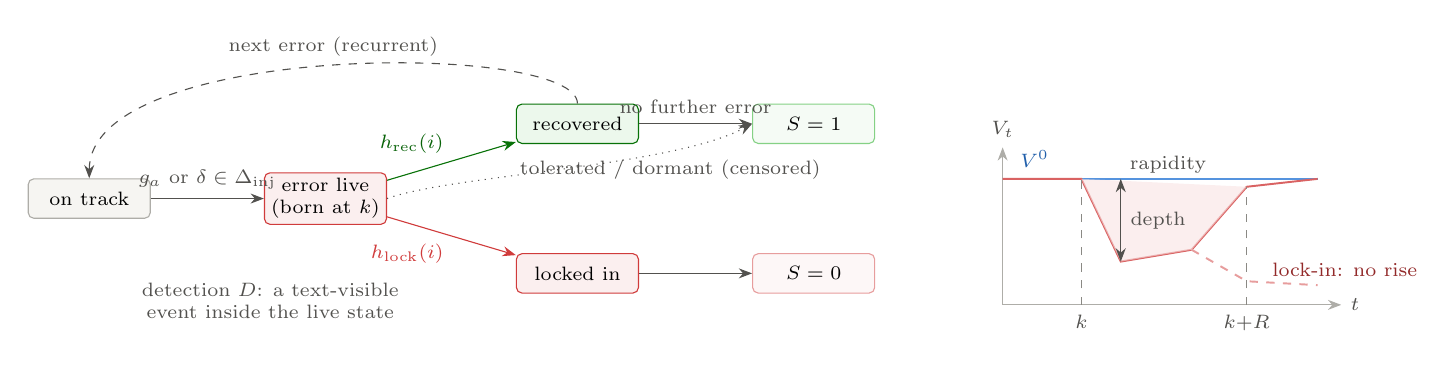
\begin{tikzpicture}[x=1cm,y=1cm,font=\scriptsize,>=Stealth,
  st/.style={draw=rule!80!black,fill=surface,rounded corners=2pt,minimum height=0.5cm,minimum width=1.55cm,inner sep=2pt,align=center},
  bad/.style={draw=critical,fill=critical!8,rounded corners=2pt,minimum height=0.5cm,minimum width=1.55cm,inner sep=2pt,align=center},
  ok/.style={draw=good!70!black,fill=good!8,rounded corners=2pt,minimum height=0.5cm,minimum width=1.55cm,inner sep=2pt,align=center}]
% multi-state diagram
\node[st] (track) at (0,0) {on track};
\node[bad] (live) at (3.0,0) {error live\\(born at $k$)};
\node[ok] (rec) at (6.2,0.95) {recovered};
\node[bad] (lock) at (6.2,-0.95) {locked in};
\node[ok,draw=good!50,fill=good!4] (succ) at (9.2,0.95) {$S=1$};
\node[bad,draw=critical!50,fill=critical!4] (fail) at (9.2,-0.95) {$S=0$};
\draw[->,ink2] (track) -- node[above,text=ink2]{$g_a$ or $\delta\in\Delta_{\mathrm{inj}}$} (live);
\draw[->,good!70!black] (live) -- node[above left=-1pt,text=good!60!black]{$h_{\mathrm{rec}}(i)$} (rec);
\draw[->,critical] (live) -- node[below left=-1pt,text=critical]{$h_{\mathrm{lock}}(i)$} (lock);
\draw[->,ink2] (rec) -- node[above,text=ink2]{no further error} (succ);
\draw[->,ink2] (lock) -- (fail);
\draw[->,ink2,dashed] (rec.north) .. controls (6.2,2.0) and (0,2.0) .. node[above,text=ink2,pos=0.5]{next error (recurrent)} (track.north);
\draw[->,ink2,dotted] (live.east) .. controls (4.6,0.3) and (7.4,0.4) .. node[below,text=ink2,pos=0.75]{tolerated / dormant (censored)} (succ.west);
\node[text=ink2,align=center,anchor=north] at (2.3,-0.95) {detection $D$: a text-visible\\event inside the live state};
% value curve with resilience triangle
\begin{scope}[shift={(11.6,-1.35)}]
\draw[->,rule!80!black] (0,0) -- (4.3,0) node[right,text=ink2]{$t$};
\draw[->,rule!80!black] (0,0) -- (0,2.0) node[above,text=ink2]{$V_t$};
\draw[s1!80,line width=0.7pt] (0,1.6) -- (4.0,1.6);
\draw[critical!80,line width=0.7pt] (0,1.6) -- (1.0,1.6) -- (1.5,0.55) -- (2.4,0.7) -- (3.1,1.5) -- (4.0,1.6);
\draw[critical!50,line width=0.7pt,dashed] (2.4,0.7) -- (3.1,0.3) -- (4.0,0.25);
\fill[critical!15,opacity=0.6] (1.0,1.6) -- (1.5,0.55) -- (2.4,0.7) -- (3.1,1.5) -- cycle;
\draw[ink3,dashed] (1.0,0) -- (1.0,1.6) node[below,at start,text=ink2]{$k$};
\draw[ink3,dashed] (3.1,0) -- (3.1,1.5) node[below,at start,text=ink2]{$k{+}R$};
\draw[<->,ink2] (1.5,0.55) -- (1.5,1.6) node[midway,right,text=ink2]{depth};
\node[text=ink2] at (2.1,1.78) {rapidity};
\node[text=critical!70!black,anchor=west] at (3.3,0.45) {lock-in: no rise};
\node[text=s1!80!black,anchor=west] at (0.1,1.85) {$V^0$};
\end{scope}
\end{tikzpicture}
\caption{Left: the multi-state model of an error's lifetime (Definition~\ref{def:lifetime}). The live state is exited by recovery or lock-in with competing hazards; a run that ends with the error live but harmless is a censored observation. Proposal~2's hazard model is the special case without the recovery transition. Right: the same on the success-probability curve $V_t$ of the prefix (Definition~\ref{def:resilience}): recovery is a dip followed by a rise, lock-in a dip without one, and the shaded area is the resilience loss $\mathcal{R}$ with its depth and rapidity.}
\label{fig:lifecycle}
\end{figure}

\begin{rqbox}{4}
\begin{description}[leftmargin=3.2em,style=sameline,font=\bfseries,itemsep=1.5pt]
\item[RQ\,4.1] What are the cumulative incidences of recovery and lock-in, and the detection-latency distribution, as functions of the lag after an injected error, and how do they depend on position, error mode, fault side and system? Is the one-step median fix window of natural failures also the recovery time of injected errors, or is it a selection effect of failed runs?
\item[RQ\,4.2] What fraction of absorption is dormancy, masking, correction and overwriting, given that only the last two are the hypothesised capability and the first two are task slack?
\item[RQ\,4.3] Is the fragility curve a step function aligned with the system's verification checkpoints, and does removing or adding a verifier move it by the coverage the checkpoint model predicts?
\item[RQ\,4.4] How often is an error recovered without ever being detected, and does a detected-but-unfixed error look different in the text from one that was never detected?
\item[RQ\,4.5] What are the generation, permeability, containment and exposure rates of the agent roles in the surveyed systems, is the spectral radius of the propagation matrix below one, and does the branching-process absorption probability predict the measured coverage?
\item[RQ\,4.6] How does the probability of a fatal outcome grow with the severity of an injected error, and is there a critical severity per position---the basin size of the resilience picture?
\item[RQ\,4.7] For two injected errors, is the joint effect independent, compounding, or protective, in the sense that the first error triggers a check that catches the second?
\item[RQ\,4.8] What does a recovered error cost in steps and tokens, and is recovering in place cheaper than restarting from the prefix before the error?
\item[RQ\,4.9] Can a recovered error be found from the log alone, without rollouts, from the dip-and-rise signature of a learned success-probability curve or from a hidden state that switches back, and with what delay can an online monitor tell a transient dip from a lock-in?
\end{description}
\end{rqbox}

\begin{multicols}{2}
\paragraph{Experiments}
\begin{description}[leftmargin=1.4em,style=nextline,itemsep=1pt]
\item[\EXP{4.1} --- Fate screen (answers \RQ{4.2}, \RQ{4.4}; supplies \RQ{4.1}, \RQ{4.8}).] The injection half of \EXP{1.1} with every continuation \emph{kept} and labelled with Definition~\ref{def:fate}. The consumption test is a second, cheap counterfactual: for each step $k{+}i$ of $\omega$, re-issue that single LLM call with $\delta(s_k)$ removed from its context and compare the output (one call per step, not a rollout). Detection $D$ is a judge pass over the text with the injection known; recovery $R$ is the first lag at which the consumption test stays negative for the rest of the run and $V^\delta$ has returned to $V^0-\alpha$; lock-in $L$ is estimated by the surrogate of \EXP{1.2} and verified by rollouts on a subset. Output: the fate distribution per system, mode, position and fault side, the triples $(D,R,L)$ with censoring indicators, and the resilience loss $\mathcal{R}$ with its depth and rapidity.
\item[\EXP{4.2} --- Lifetime curves (answers \RQ{4.1}, \RQ{4.8}).] On the output of \EXP{4.1}, Aalen--Johansen cumulative incidences \cite{aalen1978empirical} for recovery and lock-in, then a multi-state Cox model \cite{andersen1982cox,putter2007multistate} with position, mode, fault side, system and checkpoint distance as covariates, and a shared frailty per agent and per task \cite{vaupel1979frailty}. Validation on natural labels: $t_{\mathrm{obs}}-t_{\mathrm{err}}$ and $t_{\mathrm{lock}}-t_{\mathrm{err}}$ of the 1,184 Failure-as-a-Process failures, the detour length and recovery count of its 610 passes, and AgentRx's recovered events.
\item[\EXP{4.3} --- Checkpoint ablation (answers \RQ{4.3}).] Align $r(k/T)$ with $\mathcal{C}(\tau)$ in systems with an explicit verifier (Magentic-One's ledger, LongRCA's verification expert, the test runs of SWE agents), then remove, add or delay the verifier and re-run \EXP{4.1}. The checkpoint model predicts the shift; the alternative---recovery driven by observations rather than by designated checks---predicts none.
\item[\EXP{4.4} --- Propagation matrix (answers \RQ{4.5}).] On the MASLab systems of row 4 of Table~\ref{tab:engine}, inject at the output of agent $a$ and judge the wrongness of each consuming agent's next output against the unperturbed branch; estimate $M_{ab}$, $\rho(M)$ and the branching-process absorption probability, and compare with the measured $C$. The same data give $(g_a,\pi_a,c_a,x_a)$ per role.
\item[\EXP{4.5} --- Dose and interaction (answers \RQ{4.6}, \RQ{4.7}).] Severity-graded injectors $\delta_\sigma$ (size of a numeric error, fraction of a page truncated, number of corrupted arguments) and paired injections at $(k_1,k_2)$ on the same prefixes as \EXP{4.1}; report $\sigma^\star(k)$ and the interaction term $\log p_{\delta_1\delta_2}-\log p_{\delta_1}-\log p_{\delta_2}+\log p_0$.
\item[\EXP{4.6} --- Recovered-error detection from logs (answers \RQ{4.9}).] Train on outcome-only data (level L1 of Definition~\ref{def:levels}) a hidden semi-Markov model \cite{yu2010hsmm} with an ``error live'' state that can switch back, and a value curve $V_t$ with a temporal-difference consistency loss, and score recovery segments against the four released sources of recovered errors: Failure-as-a-Process passes, AgentRx non-root events (\S\ref{ds:agentrx}), TRAIL traces that end correctly but carry error spans (\S\ref{ds:trail}) and MP-Bench steps flagged by one annotator of three (\S\ref{ds:mp_bench}).
\item[\EXP{4.7} --- Online monitor with a delay guarantee (answers \RQ{4.9}).] A CUSUM \cite{page1954cusum} on the hazard or value sequence of \EXP{2.3}, scored by lead time to $t_{\mathrm{lock}}$ and by false alarms on passes with recovered errors, the hardest negatives; the Lorden delay--false-alarm bound \cite{lorden1971} gives the curve a monitor cannot beat.
\end{description}
\end{multicols}

\medskip\noindent\begin{minipage}{\linewidth}\centering\scriptsize
\setlength{\tabcolsep}{3pt}
\begin{tabularx}{\linewidth}{@{}l >{\RaggedRight\hsize=1.25\hsize}X >{\RaggedRight\hsize=0.95\hsize}X >{\RaggedRight\hsize=0.8\hsize}X@{}}\toprule
Exp. & Data & Metrics & Baselines / reference values \\\midrule
\EXP{4.1} & \emph{Collected}: the injected continuations of \EXP{1.1} on rows 1--5 of Table~\ref{tab:engine}, kept whether or not they fail, injected uniformly over position; one extra LLM call per continuation step for the consumption test; a judge pass for $D$ & fate distribution per system, mode, position and fault side; $(D,R,L)$ with censoring indicators; inter-judge agreement on $D$ ($\kappa$); dormant fraction per injector; $\mathcal{R}$, depth and rapidity & Aegis absorption 23--66\% as the undecomposed $C$; Inspector-agent recovery 96.4\% \cite{huang2024resilience}; cascade attenuation 0.422 $\to$ 0.272 \cite{jamshidi2026cascade} \\
\EXP{4.2} & output of \EXP{4.1}; \emph{natural validation}: Failure-as-a-Process FAIL ($t_{\mathrm{err}}/t_{\mathrm{lock}}/t_{\mathrm{obs}}$, recovery attempts, 1,184) and PASS (first error step, recoveries, detour length, 610); AgentRx recovered events & $F_{\mathrm{rec}}(i)$, $F_{\mathrm{lock}}(i)$ and $P_{\mathrm{detect}}$ with confidence bands; hazard ratios of the Cox covariates; frailty variance per agent and task; agreement in \emph{shape} between injected and natural curves & natural fix-window distribution (median 1, 239 runs $>10$); awareness classes (58.7\% unaware, 34.9\% wrong fix) \\
\EXP{4.3} & systems with an explicit verifier (Magentic-One ledger, LongRCA verification expert, SWE-agent test runs), with the verifier removed, added or delayed & shift of $r(k/T)$ at the checkpoint positions; estimated $c_j$ per checkpoint; goodness of fit of the step-function model against a smooth decay & checkpoint null model versus the observation-driven alternative (no shift) \\
\EXP{4.4} & MASLab systems of row 4 (LLM Debate, MacNet, AgentVerse, DyLAN, Magentic-One); injections at each agent's output; judge of downstream wrongness against ground truth and unperturbed samples & $(g_a,\pi_a,c_a,x_a)$ per role; $M_{ab}$ and $\rho(M)$; predicted versus measured absorption probability; ranking of agents to harden & hierarchical-vs-flat loss of \citet{huang2024resilience}; Aegis-Bench (agent, mode) labels for $g_a$ \\
\EXP{4.5} & same prefixes as \EXP{4.1}; severity ladder with 4--5 levels per injector; pairs $(k_1,k_2)$ at fixed distances & $\Pr[\text{fatal}\mid\sigma]$ and $\sigma^\star(k)$ at threshold 0.5; interaction term with its sign and interval & independence (zero interaction); minimal repair families \cite{li2026mrfr} for the repair side \\
\EXP{4.6} & \emph{train}: outcome-only corpora of Proposal~2; \emph{test}: Failure-as-a-Process passes (610), AgentRx non-root events, TRAIL correct-ending traces with error spans, MP-Bench one-of-three steps & recall of recovered errors and of fatal errors reported separately; segment overlap (IoU) with annotated detours; precision on clean passes & \textsc{Oat} and the one-class detectors (expected to flag recovered and fatal errors alike); Proposal~2's hazard model without the return transition \\
\EXP{4.7} & Failure-as-a-Process FAIL ($t_{\mathrm{lock}}$) and PASS runs with recovered errors; Magentic-One ledger traces & detection delay versus false-alarm rate (the full curve); median lead time to $t_{\mathrm{lock}}$; false alarms on recovered-error passes & Lorden bound \cite{lorden1971}; Failure-as-a-Process prompted monitor (82\% precision, 18\% recall, lead time 0); \EXP{2.3} without CUSUM \\\bottomrule
\end{tabularx}
\captionof{table}{Evaluation of Proposal 4: data, metrics and baselines per experiment.}
\label{tab:eval_p4}
\end{minipage}\medskip

\begin{multicols}{2}
\paragraph{Evaluation: data and metrics} Table~\ref{tab:eval_p4} lists them per experiment; three conventions apply.
\begin{itemize}[leftmargin=1.1em]
\item \emph{Survival estimators, not averages.} Every lifetime quantity is estimated with censoring handled (Aalen--Johansen, Cox), because a run that ends with the error live and $S{=}1$ carries no $R$ and no $L$.
\item \emph{Detection is a judgement, recovery is a measurement.} $D$ depends on a judge reading the text; $R$ and $L$ are counterfactual. Inter-judge agreement on $D$ is reported, and $D$ never defines the fate.
\item \emph{Natural labels validate shape, not location.} $t_{\mathrm{obs}}$ can precede $t_{\mathrm{lock}}$ in Failure-as-a-Process and judge labels drift to the symptom \cite{shen2026epv}, so the natural curves are compared with the injected ones in shape.
\end{itemize}

\paragraph{Feasibility with the surveyed data}
\begin{itemize}[leftmargin=1.1em]
\item \emph{Released recovered errors} (for \EXP{4.2} validation and \EXP{4.6}): Failure-as-a-Process ships, per PASS run, the first error step, the number of error events and recoveries, the maximal detour length and a near-miss flag, and per FAIL run $t_{\mathrm{err}}/t_{\mathrm{lock}}/t_{\mathrm{obs}}$, the number of recovery attempts, forewarning signals and the awareness class; AgentRx annotates every failure event including the recovered ones (up to 55 per trajectory); TRAIL's 148 runs are not selected by outcome; MP-Bench's three votes per step separate consensus errors from minority ones. No new annotation is needed on the natural side.
\item \emph{Injected side.} Aegis reports absorption rates but ships no absorbed branches, and Who\&When~Pro and TracerTraj discard them likewise, so \EXP{4.1} is a re-run of the released injectors (Aegis's factory, Who\&When~Pro's injector) with the negatives kept, on rows 1--5 of Table~\ref{tab:engine}; row 4 (MASLab systems, no environment state) is the cheapest and the natural home of \EXP{4.4}.
\item \emph{Budget.} \EXP{4.1} reuses the $\approx$25\,k continuations of \EXP{1.1} and adds one call per continuation step ($\approx10^6$ calls, below the rollout cost); \EXP{4.2}, \EXP{4.6} and \EXP{4.7} are statistical fits on the result; \EXP{4.3}--\EXP{4.5} multiply the injection side by the number of ablations and severities (3--5$\times$) on a subset of prefixes.
\end{itemize}

\paragraph{Pitfalls to design for}
\begin{itemize}[leftmargin=1.1em]
\item \emph{Censoring.} Short runs (ALFWorld's 30-step cap) censor heavily; naive fractions over observed events are biased.
\item \emph{Dormancy inflates coverage.} An injection into content the task never needs is absorbed trivially; Definition~\ref{def:fate} separates it, and the dormant fraction per injector is itself a result about the injectors of Section~\ref{sec:g2}.
\item \emph{Baseline stochasticity.} 39 of 54 successful MAS runs fail at least once in three reruns \cite{luan2026symtrace}, so $V^0$ is a curve with intervals, and ``fatal'' is a drop relative to it, not an absolute failure.
\item \emph{Wrongness of downstream outputs} (\EXP{4.4}) needs a reference: the unperturbed branch is stochastic, so the judge compares against the ground truth or a sample of unperturbed continuations, with the same caveat as $D$.
\item \emph{Injector realism and position prior.} The released injectors place errors late (Fig.~\ref{fig:errpos}); inject uniformly over positions and stratify every curve by $k/T$, or the lifetime curves inherit the prior.
\end{itemize}

\paragraph{What would count as a result}
\begin{itemize}[leftmargin=1.1em]
\item The first measured lifetime curves of errors in agent systems: recovery and lock-in incidences by lag, position, mode and system, with the fraction of absorption that is genuine correction rather than task slack.
\item A tested checkpoint model: either $r(k/T)$ is a step function that a verifier ablation shifts by the predicted amount, or recovery is observation-driven and verifier agents are not where robustness comes from.
\item Per-agent profiles $(g_a,\pi_a,c_a,x_a)$ for the roles of the surveyed systems and a propagation matrix whose spectral radius predicts absorption, which would turn ``which agent is responsible'' into ``which agent to harden''.
\item A label-free detector of recovered errors with a measured delay--false-alarm curve for the online monitor, placed against the Lorden bound.
\end{itemize}
\end{multicols}

\section{Proposal 5: Where to re-roll a single generation---the restart frontier}\label{sec:future:reroll}

\begin{multicols}{2}
\paragraph{Motivation} Proposals 1--4 ask which step of a failed run \emph{matters}. This proposal asks the operational question that follows once an attributor has answered: given a failed multi-step generation and a budget of tokens, \emph{from which step should the generation be re-rolled}? It is posed in the simplest setting that has the structure of the problem---one model, one generation, no environment---because there every quantity of Section~\ref{sec:future:prelim} can be measured exactly and cheaply, and because the setting is the pilot that Proposal~1 needs before it pays for agent rollouts. Four observations make the question non-trivial.
\begin{itemize}[leftmargin=1.1em]
\item \emph{The best position is not the earliest.} On ALFWorld and WebShop the net gain of a single-step repair differs by 0.51 on average across the thirds of a trajectory, and the earliest-single-success rule of AgenTracer loses up to 0.58 against the best position \cite{liao2026repairs}. On SWE-bench, restarting from the judge-labelled step changes success by $-0.03$ to $-0.08$ while restarting from the certified point of no return raises it from 0.44 to 0.53 \cite{shen2026epv}. Earliest-step labels (Who\&When, TrajErrBench, LongRCA) and first-error labels (ProcessBench \cite{zheng2024processbench}, PRM800K) are therefore not restart recommendations.
\item \emph{Restart value is concentrated and often late.} On MATH-500 chains of DeepSeek-R1-Distill-Qwen-14B the gain of restarting at a step is concentrated in a few positions (pooled Gini 0.896) and a trained position selector does not beat the rule ``restart from the last eligible steps'' \cite{atri2026expanding}. The fix window $t_{\mathrm{lock}}-t_{\mathrm{err}}$ of Failure-as-a-Process has median 1 step (\S\ref{ds:failure_as_process}), so in agent runs the set of positions from which a re-roll helps can be a single step.
\item \emph{Position is worth several points, and nobody has priced it.} Entropy-guided choice of the cut point moves MATH500 accuracy of Qwen2.5-Math-7B between 72.6 (random cut) and 77.6 (gradient-traced cut) at $\approx9\times$ the tokens of a single pass \cite{ding2026rewind}; keeping the steps before the first verifier-flagged step and regenerating the rest reaches a higher accuracy than Best-of-10 with 77.8\% fewer tokens \cite{wu2024stepco}; a learned backtracking token rewinds one step at inference and adds 2.9 points over no rewind \cite{yang2025selfbacktrack}. Each study fixes one position rule and reports either accuracy or tokens; none reports the two as a function of the position.
\item \emph{A re-roll can also destroy a correct answer.} Unconditional revision overturns 19.1\% of the initially correct GSM8K answers of Llama-3.1-8B while raising accuracy by 25.5 points \cite{zhang2026riskaware}; conditioning a retry on the previous attempt makes small code models reproduce a near-identical program in 33--68\% of retries against 2--14\% for a blind resample, and the blind resample wins at 2.5--5.5$\times$ fewer tokens \cite{verma2026tryagain}. Whether \emph{keeping a prefix} inherits this anchoring, and whether later restarts break fewer correct runs, is unmeasured.
\end{itemize}
The proposal therefore treats the re-roll position as a decision with two axes---the success probability it buys and the tokens it spends---and measures the frontier between them on failed \emph{and} successful generations.

\paragraph{Closest prior work} Six strands contain parts of the programme; Table~\ref{tab:rules} collects the position rules they use, which become the baselines of \EXP{5.2}.
\begin{itemize}[leftmargin=1.1em]
\item \emph{Prefix value curves.} OmegaPRM \cite{luo2024omegaprm} estimates the success rate of every prefix by Monte-Carlo continuation and labels the first collapse; Thought Anchors and Thought Branches \cite{bogdan2025thoughtanchors,macar2025thoughtbranches} resample each sentence of a long chain of thought 100 times and read the shift in the answer distribution; EPV \cite{shen2026epv} does the same on SWE-bench prefixes. These give the profile of Definition~\ref{def:restart} below but not its cost, and they are read as attribution, not as a restart rule. ``Expanding LLM Reasoning'' \cite{atri2026expanding} is the exception that trains a position selector on restart value; it restricts restarts to the last third of a chain, scores cost as aggregate output and finds its selector no better than always-last.
\item \emph{Cut-point regeneration.} Power sampling \cite{karan2026power} regenerates a suffix from a uniformly random cut and accepts by likelihood; REWIND \cite{ding2026rewind} and entropy-cut Metropolis--Hastings \cite{zhou2026entropycut} choose the cut at an entropy rise, the latter proving that mixing time then scales with the number of decisions rather than tokens; CUSUM re-decoding \cite{ettifouri2026cusum} rolls back to a saved KV state on an alarm and reports that rolling back \emph{without changing the continuation} is insufficient. REWIND contains the only cut-rule ablation on single-model reasoning; none of the four reports accuracy against position-dependent cost.
\item \emph{First-error rules.} StepCo \cite{wu2024stepco} regenerates from the first step a process verifier scores below a threshold; HPFA \cite{zhu2026hpfa} labels the root cause as the earliest step whose replacement plus resampling succeeds; InT \cite{yang2026int} has the model propose a fix at its first error; ELPO \cite{liang2026elpo} binary-searches the first irrecoverable step. All four commit to \emph{earliest}, which the agent-side evidence above argues against.
\item \emph{Restarts inside training.} Thinking Seeds \cite{yang2026thinkingseeds} restarts on-policy RL from truncated prefixes at a fixed length ratio (an entropy-chosen cut did worse) and names adaptive restart selection as future work; Re$^2$ \cite{wang2026resolve} trains the model to decide between continuing and re-solving from scratch; Proposal~3's restart entry point~R (Table~\ref{tab:entry}) is the agent version. None of them chooses the position by its measured value.
\item \emph{Self-correction accounting.} The decomposition of a re-roll into keeping correct answers and fixing wrong ones \cite{yang2024confcrit,huang2024cannot,kamoi2024survey}, the closed-form ceiling of iterated re-rolling $\mathrm{CS}/(1-\mathrm{CL}+\mathrm{CS})$ \cite{yang2025scaling}, SCoRe's $\Delta(i{\to}c)$, $\Delta(c{\to}i)$ \cite{kumar2025score} and the harm and recovery rates of \citet{zhang2026riskaware} supply the metrics of Definition~\ref{def:restart}; selective verification \cite{dip2026thinkagain} and anchoring \cite{verma2026tryagain} supply the operator baselines of \EXP{5.3}. All of them re-roll the \emph{whole} answer; none has a position.
\item \emph{Agents.} Rollback-induced reflection \cite{yu2026rir} restores the latest checkpoint that removes the failure condition while preserving valid progress, which is the rule this proposal makes measurable, on the joint checkpoints that AgentRewind \cite{zhuang2026agentrewind} provides; CausalFlow \cite{bonagiri2026causalflow} scores minimality of a repair but states that plain chains of thought ``provide no identifiable intervention points''; \citet{liao2026repairs} show that the best position depends on who continues the run.
\end{itemize}
What is missing from all of them is the pair $(p(k),c(k))$ on the same trajectories, the retention side on successful trajectories, and a comparison of position rules and re-roll operators at matched regenerated tokens.
\end{multicols}

\begin{table}[h]\centering\small
\begin{tabularx}{\linewidth}{@{}>{\RaggedRight\hsize=0.75\hsize}X >{\RaggedRight\hsize=1.35\hsize}X >{\RaggedRight\hsize=0.9\hsize}X@{}}\toprule
Position rule & Definition (restart from step $k$) & Source \\\midrule
\textsc{none} & $k=T{+}1$: keep the generation as it is & reference point $p(T{+}1)=S(\tau)$ \\
\textsc{blind} & $k=1$: resample from the question & \citet{verma2026tryagain}; self-consistency \\
\textsc{uniform} & $k$ drawn uniformly from $\{1,\dots,T\}$ & power sampling \cite{karan2026power} \\
\textsc{always-last} & the last eligible step (last third of the chain) & \citet{atri2026expanding} \\
\textsc{one-back} & $k=T$: regenerate the last step only & Self-Backtracking at inference \cite{yang2025selfbacktrack} \\
\textsc{first-flag} & first step whose process-verifier score falls below a threshold & StepCo \cite{wu2024stepco}, Math-Shepherd \cite{wang2024mathshepherd} \\
\textsc{human-first} & the human first-error label & ProcessBench \cite{zheng2024processbench}, PRM800K \cite{lightman2023prm} \\
\textsc{entropy-cut} & largest adjacent entropy rise in a window before the entropy peak, aligned to a delimiter & REWIND \cite{ding2026rewind}, \citet{zhou2026entropycut} \\
\textsc{largest-drop} & $\arg\max_k\,[p(k)-p(k{+}1)]$ on the value curve & OmegaPRM \cite{luo2024omegaprm}, EPV \cite{shen2026epv} \\
\textsc{earliest-fix} & smallest $k$ with $p(k)\ge\alpha$ & HPFA \cite{zhu2026hpfa}; $k^\star$ of Definition~\ref{def:fa} \\
\textsc{max-effect} & $\arg\max_k p(k)$ & Proposal~1 \\
\textsc{latest-}$\varepsilon$ & largest $k$ with $p(k)\ge\max_j p(j)-\varepsilon$ & this proposal (Definition~\ref{def:frontier}) \\
\textsc{oracle} & the frontier of Definition~\ref{def:frontier} from the rollouts themselves & ceiling \\\bottomrule
\end{tabularx}
\caption{Position rules compared in \EXP{5.2}. Rules above the midrule need no rollouts; the three below it need the restart profile and are what a predictor (\EXP{5.4}) tries to approximate.}
\label{tab:rules}
\end{table}

\begin{multicols}{2}
\paragraph{Setting} One model $\pi$ with a fixed decoding configuration (sampler, temperature, thinking budget) answers a task $x$ with an automatic success predicate $S$ (reference answer, unit tests). Its generation is $\tau=(s_1,\dots,s_T)$, where a step is a sentence or a delimited reasoning step as in Thought Anchors \cite{bogdan2025thoughtanchors}, and the final answer is part of $s_T$. There is no environment, so Assumption~\ref{as:replay} holds trivially and $\mathrm{Roll}(\tau_{<k})$ is the model's own continuation from the kept prefix. The intervention is the one entry missing from Table~\ref{tab:vocab}: \textsc{resample}, which replaces $s_k$ and everything after it by a fresh draw of $\pi$.

\begin{definition}{Restart profile and restart cost}{restart}
For a generation $\tau$ and a position $k\in\{1,\dots,T{+}1\}$, the \emph{restart} $R_k(\tau)=\mathrm{Roll}(\tau_{<k})$ keeps $s_1,\dots,s_{k-1}$ and regenerates the rest; $R_1$ is a blind resample and $R_{T+1}$ is the original generation. Its \emph{restart profile} and \emph{restart cost} are
\begin{align*}
p_\tau(k)&=\Pr\big[S(R_k(\tau))=1\big],\\
c_\tau(k)&=\mathbb{E}\big[\,\#\text{tokens generated by }R_k(\tau)\big],
\end{align*}
both estimated from $N$ independent restarts; $p_\tau(k)=p_0(\tau,k{-}1)$ in the notation of Definition~\ref{def:effect}, i.e.\ the profile is the prefix-value curve of Proposal~1 read at every position. On a failed generation $p_\tau$ is the \emph{recovery} curve and $p_\tau(k)-p_\tau(T{+}1)$ the gain of restarting at $k$; on a successful generation $p_\tau$ is the \emph{retention} curve and $1-p_\tau(k)$ the harm. Averaged over a corpus, recovery and retention are the critique score and the confidence level of \citet{yang2024confcrit} indexed by position.
\end{definition}

\begin{definition}{Restart frontier and position rules}{frontier}
The \emph{restart frontier} of $\tau$ is the set of positions not dominated in $(p_\tau(k),-c_\tau(k))$. Three scalar rules read it:
\begin{itemize}[leftmargin=1.1em]
\item \textsc{max-effect} $k_{\max}=\arg\max_k p_\tau(k)$;
\item \textsc{latest-}$\varepsilon$ $k_\varepsilon=\max\{k:\ p_\tau(k)\ge p_\tau(k_{\max})-\varepsilon\}$, the cheapest position within $\varepsilon$ of the best;
\item \textsc{price-}$\lambda$ $k_\lambda=\arg\max_k\,[p_\tau(k)-\lambda\,c_\tau(k)]$ for a stated price $\lambda$ per token.
\end{itemize}
The \emph{regret} of any position rule $r$ at a token budget $B$ is the difference between the success probability of the frontier at $B$ and that of $r$ at the same budget, averaged over the corpus; it is the metric of \EXP{5.2} and \EXP{5.4}. The \emph{fix window} of Definition~\ref{def:fa} reappears as $k_{\mathrm{lock}}-k_{\max}$.
\end{definition}

\begin{assumption}{Prefix fidelity}{prefix}
Restoring the prefix $\tau_{<k}$ reproduces the continuation distribution the model would have had at step $k$. Two things can break it and are stated with every number:
\begin{itemize}[leftmargin=1.1em]
\item \emph{Cache versus re-prefill.} Continuing from the retained KV cache and re-prefilling the same tokens produce different suffixes in BF16 for 166 of 200 Qwen2.5 traces, with accuracy unchanged within noise; in FP32 they agree \cite{lorup2026stagereplay}. The cost of a restart counts generated tokens; the prefill of a prefix that is not cached is reported separately.
\item \emph{Decoding.} Under greedy decoding $R_k(\tau)$ reproduces $\tau$ and the profile is degenerate; the sampler and temperature are part of the definition of $p_\tau$, as the executor is in \citet{liao2026repairs}.
\end{itemize}
\end{assumption}

Two remarks fix what is and is not new in the objects. The profile $p_\tau$ is the value curve that Proposals 1, 2 and 3 already estimate (the \textsc{resample} column of \EXP{1.1}, the survival function $\bar S_t$ of Proposal~2, the restart point of Proposal~3), so the measurement is shared. What is new is the second axis $c_\tau$, the retention side, and the rules of Definition~\ref{def:frontier}: under a near-flat profile---which the concentration result of \citet{atri2026expanding} and the median fix window of one step both predict to be common---\textsc{max-effect} and \textsc{earliest-fix} pick an early, expensive position, and \textsc{latest-}$\varepsilon$ is the rule that resolves the tension between effectiveness and efficiency explicitly.
\end{multicols}

\begin{rqbox}{5}
\begin{description}[leftmargin=3.2em,style=sameline,font=\bfseries,itemsep=1.5pt]
\item[RQ\,5.1] For a failed single-model generation, how does the success probability of a restart depend on the position it is restarted from, how concentrated is the gain, and how wide is the window of positions that recover the run?
\item[RQ\,5.2] When several positions recover the run with near-equal probability, how much cheaper is the latest of them, and what regret do the position rules of Table~\ref{tab:rules} incur against the frontier at a matched token budget?
\item[RQ\,5.3] Does restarting a correct generation keep its answer, does retention rise with the restart position, and is the harm of a restart smaller than the harm of a whole-answer revision?
\item[RQ\,5.4] Is a kept prefix worth keeping: at matched regenerated tokens, does a prefix restart beat a blind resample and a rewrite conditioned on the whole generation, and when does the kept prefix anchor the continuation to the original error?
\item[RQ\,5.5] Can the frontier position be predicted from the prefix---token entropy, verifier scores, hidden states, verbalised confidence---well enough to choose it without rollouts, and does the predictor beat always-last, first-flag and entropy-cut?
\item[RQ\,5.6] Do restart profiles of single-model generations have the same shape as the \textsc{resample} profiles of agent trajectories, so that the single-model setting is a valid pilot for Proposal~1?
\end{description}
\end{rqbox}

\begin{multicols}{2}
\paragraph{Experiments}
\begin{description}[leftmargin=1.4em,style=nextline,itemsep=1pt]
\item[\EXP{5.1} --- The restart profile (answers \RQ{5.1}, \RQ{5.3}).] For each model and task, sample one generation per problem at the model's default temperature, keep the failed and the successful ones in equal numbers, and restart every generation at each step boundary (all boundaries when $T\le40$, else 16 positions at length quantiles plus the human first-error step where one exists) with $N=16$ continuations per position; record $S$ and the number of generated tokens. Estimate $p_\tau$ and $c_\tau$ with intervals, the Gini concentration of the gain, $k_{\max}$, $k_\varepsilon$ for $\varepsilon\in\{0.05,0.1\}$, the window $\{k:p_\tau(k)\ge p_\tau(k_{\max})-\varepsilon\}$ and, on successful generations, the retention curve. Every continuation is stored; \EXP{5.2}--\EXP{5.4} are computed on it.
\item[\EXP{5.2} --- Rules against the frontier (answers \RQ{5.2}).] Apply every rule of Table~\ref{tab:rules} to the profiles of \EXP{5.1}, compute each rule's success probability and expected tokens, and its regret against the frontier at matched budgets $B$; report the gain per regenerated token of each rule and the token saving of \textsc{latest-}$\varepsilon$ over \textsc{max-effect} and \textsc{earliest-fix} at equal success. Human first-error labels are scored here as a position rule, which answers for ProcessBench and PRM800K the question \EXP{1.3} asks of the agent labels.
\item[\EXP{5.3} --- Operators at matched tokens (answers \RQ{5.4}).] At the positions chosen by \textsc{latest-}$\varepsilon$ and \textsc{max-effect}, compare four re-roll operators at equal regenerated tokens: the prefix restart $R_k$; a blind resample $R_1$ with the same budget (several draws, majority vote); a rewrite conditioned on the whole generation, with and without the content-free ``this may be wrong'' placebo of \citet{verma2026tryagain}; and $R_k$ preceded by a \textsc{hint} at $k$ (Table~\ref{tab:vocab}) as the information-rich ceiling. Measure recovery, retention, the near-duplicate rate between the regenerated and the original suffix, and whether the regenerated suffix reproduces the original error (resilience in the sense of \citet{macar2025thoughtbranches}).
\item[\EXP{5.4} --- Predicting the position (answers \RQ{5.5}).] Train a listwise position selector on the frontier labels of \EXP{5.1} from prefix features---per-token entropy and its rise, process-verifier scores, a linear probe on hidden states \cite{yuan2026hiddenerror}, verbalised confidence---with ties between positions broken at random \cite{atri2026expanding}; test on held-out problems, held-out tasks and a held-out model; score it as a rule in \EXP{5.2}'s terms. The surrogate of Proposal~1 (Definition~\ref{def:surrogate}) is trained on the same tuples and scored alongside.
\item[\EXP{5.5} --- Transfer to agents (answers \RQ{5.6}).] Run the \textsc{resample} intervention of \EXP{1.1} at all positions on rows 1--2 of Table~\ref{tab:engine} ($\tau^2$-Bench, ALFWorld) with $N=8$, and compare the shape statistics of the profiles---Gini concentration, $k_\varepsilon/T$, window width, retention slope---with those of \EXP{5.1}; report where the single-model shapes predict the agent shapes and where the environment (irreversible actions, tool state) breaks the correspondence.
\end{description}
\end{multicols}

\medskip\noindent\begin{minipage}{\linewidth}\centering\scriptsize
\setlength{\tabcolsep}{3pt}
\begin{tabularx}{\linewidth}{@{}l >{\RaggedRight\hsize=1.2\hsize}X >{\RaggedRight\hsize=0.95\hsize}X >{\RaggedRight\hsize=0.85\hsize}X@{}}\toprule
Exp. & Data & Metrics & Baselines / reference values \\\midrule
\EXP{5.1} & \emph{Collected}: 300 failed + 300 successful generations per model on MATH-500, AIME 2024--25, GPQA-Diamond, MBPP+ and HumanEval+ (unit tests give $S$); models Qwen3-4B / 8B (thinking on and off), DeepSeek-R1-Distill-Qwen-7B, Qwen2.5-Math-7B; ProcessBench (3,400 human first-error labels) and PRM800K as the labelled subset; $N=16$ per position & $p_\tau(k)$, $c_\tau(k)$ with Wilson intervals; Gini of the gain; $k_{\max}$, $k_\varepsilon$, window width in steps and in $k/T$; retention curve and harm $1-p_\tau(k)$ on successes; corpus-level critique score and confidence level per position \cite{yang2024confcrit} & no baseline (measurement); concentration Gini 0.896 and always-last of \citet{atri2026expanding}; sentence-level anchor importance of \citet{bogdan2025thoughtanchors}; harm rate 19.1\% and recovery 25.5 pts of whole-answer revision \cite{zhang2026riskaware} \\
\EXP{5.2} & profiles of \EXP{5.1}; process verifier Math-Shepherd / Qwen2.5-Math-PRM for \textsc{first-flag}; REWIND's cut rule re-implemented; ProcessBench and PRM800K labels for \textsc{human-first} & success and expected tokens per rule; regret against the frontier at $B\in\{0.25,0.5,1,2\}\times$ one full generation; gain per regenerated token; token saving of \textsc{latest-}$\varepsilon$ at equal success; agreement of \textsc{human-first} with the window & every rule of Table~\ref{tab:rules}; REWIND cut-rule ablation 72.6--77.6 on MATH500 \cite{ding2026rewind}; StepCo $-77.8\%$ tokens vs Best-of-10 \cite{wu2024stepco}; self-consistency at the same budget \cite{snell2024testtime}; human--human first-error agreement of ProcessBench as the ceiling of \textsc{human-first} \\
\EXP{5.3} & continuations of \EXP{5.1} at $k_\varepsilon$ and $k_{\max}$, plus new draws for the blind, conditioned, placebo and hinted operators at equal tokens & recovery, retention, net gain at matched tokens; near-duplicate rate (suffix similarity $>0.95$); error-reproduction rate; share of gain attributable to the hint (answer leakage control) & blind resample with majority vote; Self-Refine-style conditioned rewrite; placebo of \citet{verma2026tryagain} (near-duplicates 33--68\% vs 2--14\%); SCoRe-trained self-correction where a checkpoint exists \cite{kumar2025score}; power sampling with uniform cut \cite{karan2026power} \\
\EXP{5.4} & \emph{train}: frontier labels of \EXP{5.1}; \emph{test}: held-out problems, held-out task family, held-out model & regret of the predicted position at matched budgets; recall of the window; Brier score of predicted $p_\tau(k)$; rollouts saved at fixed regret & \textsc{always-last}, \textsc{first-flag}, \textsc{entropy-cut}, \textsc{uniform}; the learned router of \citet{atri2026expanding} (no gain over always-last, $-0.006$); Proposal~1's surrogate; hidden-state probe AUROC 0.85 of \citet{yuan2026hiddenerror} as the detection reference \\
\EXP{5.5} & \emph{Collected}: 100 failed + 100 successful runs on $\tau^2$-Bench and ALFWorld (TrajErrBench, AgentErrorBench labels), \textsc{resample} at all positions, $N=8$ & same shape statistics as \EXP{5.1}; rank correlation of $k_\varepsilon/T$ and window width between settings; regret of the single-model predictor of \EXP{5.4} applied to agent prefixes & EPV restart values on SWE-bench (judge step $-0.03$ to $-0.08$, certified PNR $0.44\to0.53$) \cite{shen2026epv}; best-position spread 0.51 of \citet{liao2026repairs}; fix-window median 1 of Failure-as-a-Process \\\bottomrule
\end{tabularx}
\captionof{table}{Evaluation of Proposal 5: data, metrics and baselines per experiment.}
\label{tab:eval_p5}
\end{minipage}\medskip

\begin{multicols}{2}
\paragraph{Evaluation: data and metrics} Table~\ref{tab:eval_p5} lists them per experiment; four conventions apply.
\begin{itemize}[leftmargin=1.1em]
\item \emph{Match tokens, not calls.} Every comparison between rules or operators is made at equal regenerated tokens; a comparison at equal numbers of attempts favours whichever operator regenerates less and is the flaw that the review of refine-over-resample claims points at \cite{verma2026tryagain}. Sequential regeneration also pays a quadratic attention cost that token counts hide \cite{qin2025backtrack}, so wall-clock and FLOPs are reported for one model as a check.
\item \emph{Recovery and retention are reported as a pair}, never as a net accuracy change; a rule that recovers many failures and breaks many successes is a different object from one that does neither, and the net depends on the base rate \cite{zhang2026riskaware}.
\item \emph{Outcome, not step, defines failure.} A generation is failed if $S(\tau)=0$; a wrong step inside a successful generation is a retention case, not a failure, because reasoning models reach correct answers over persisting errors (55--78\% of injected GSM8K errors in R1 traces are never verbalised yet the answer is right \cite{phan2026critique}).
\item \emph{The continuation policy is named.} $p_\tau$ depends on the sampler, the temperature and the thinking budget; results carry them as the executor is carried in \citet{liao2026repairs}, and the same-model executor is stated as the reason the setting is cleaner than the agent one.
\end{itemize}

\paragraph{Feasibility with the surveyed data}
\begin{itemize}[leftmargin=1.1em]
\item \emph{Data and labels.} All tasks are public with automatic $S$; ProcessBench supplies 3,400 human first-error labels on four difficulty tiers and PRM800K step labels on MATH, so \textsc{human-first} needs no annotation. The survey's labelled agent sets (TrajErrBench 400, AgentErrorBench 150) score \EXP{5.5} on rows 1--2 of Table~\ref{tab:engine}.
\item \emph{Infrastructure.} Prefix restarts are the cheapest rollout there is: no environment, prefix caching in the serving stack, one model. The Thought Anchors code \cite{bogdan2025thoughtanchors} already implements sentence segmentation and per-sentence resampling; REWIND's cut rule and StepCo's verifier loop are released.
\item \emph{Budget.} 600 generations $\times$ 16 positions $\times$ $N=16$ $\times$ an average regenerated suffix of 2\,k tokens is $\approx3\times10^8$ tokens per model, i.e.\ two orders of magnitude below the agent screen of \EXP{1.1}; \EXP{5.3} adds four operators at two positions and \EXP{5.5} adds $\approx1.5\times10^8$ agent tokens on the two cheapest rows.
\end{itemize}

\paragraph{Pitfalls to design for}
\begin{itemize}[leftmargin=1.1em]
\item \emph{Step unit.} Cutting inside a sentence changes the profile: REWIND aligns cuts to delimiters and loses accuracy with windows above 20 tokens \cite{ding2026rewind}. Positions are step boundaries, and the segmentation is fixed before any rollout.
\item \emph{Resilience.} Reasoning models regenerate removed content downstream \cite{macar2025thoughtbranches}, so a restart can re-derive the original error; \EXP{5.3} measures the reproduction rate and the window of \EXP{5.1} is read with it, since a narrow window and a high reproduction rate are the same phenomenon.
\item \emph{Early-position bias.} Ties on a flat profile broken by the earliest index put a spurious early signal into any learned selector---the sign of the selector's gain flips with the tie rule in \citet{atri2026expanding}; ties are broken at random and \textsc{latest-}$\varepsilon$ is reported with its $\varepsilon$.
\item \emph{Answer leakage.} The \textsc{hint} operator of \EXP{5.3} is constructed from the reference and must not state the answer; it is the ceiling of the ladder, and the information-free operators are the result.
\item \emph{Failures by chance.} $p_\tau(T{+}1)=S(\tau)$ is one draw; a generation that failed by chance has $p_\tau(1)$ close to its success rate, so the gain is reported relative to $p_\tau(1)$ as well as to $S(\tau)$, and problems the model never solves ($p_\tau(1)\approx0$) are reported separately.
\item \emph{Cost accounting.} Discarded tokens, prefill of uncached prefixes and the quadratic cost of long prefixes are all part of the price; CUSUM re-decoding discarded $\approx$317\,k tokens across 1,500 generations while emitted length barely moved \cite{ettifouri2026cusum}. $c_\tau$ counts generated tokens and the other terms are reported beside it.
\item \emph{Cache fidelity.} BF16 re-prefill and live-cache continuations differ \cite{lorup2026stagereplay}; the restart mechanism is fixed per experiment and stated.
\end{itemize}

\paragraph{What would count as a result}
\begin{itemize}[leftmargin=1.1em]
\item Measured restart frontiers (\EXP{5.1}, \EXP{5.2}) for several models and tasks, with the width of the recovery window and the token saving of \textsc{latest-}$\varepsilon$ over \textsc{max-effect} and \textsc{earliest-fix} at equal success---the first statement of the effectiveness--efficiency trade-off of a re-roll position as a curve rather than a rule.
\item A retention curve (\EXP{5.1}) showing whether late restarts also break fewer correct generations, which would make the late position preferable on both axes, or showing the opposite, which would make the price $\lambda$ a genuine choice.
\item A matched-token answer (\EXP{5.3}) to whether a kept prefix is worth keeping, separated from anchoring and from answer leakage.
\item A position predictor (\EXP{5.4}) with its regret against the frontier and against always-last, which is the rule it must beat to be worth training.
\item Shape statistics (\EXP{5.5}) that say how far single-model profiles stand in for agent profiles, so that Proposal~1 can be piloted at single-model cost.
\end{itemize}
The quantity is shared with Proposals 1--3; what the proposal adds is the second axis and the decision it supports.
\end{multicols}

\clearpage
\bibliographystyle{plainnat}\bibliography{bib/refs_merged}
\end{document}
